\newcommand{\includepdfwithfirstpagefit}[1]{
    \includegraphics[width=\textwidth, height=\textheight, keepaspectratio]{#1}
    \includepdf[pages=2-, fitpaper=true, nup=1x1, frame=false]{#1}
}

\newcommand{\includepdfwithonepage}[1]{
    \includegraphics[width=\textwidth, height=\textheight, keepaspectratio]{#1}
}

\chapter{เอกสารเกี่ยวข้อง}

TODO add 3 and 3-4

\section{วศ.สก.-06}
\includepdfwithfirstpagefit{resources/bureaucrats/coop6.pdf}

\section{วศ.สก.-10}
\includepdfwithfirstpagefit{resources/bureaucrats/coop10.pdf}

\section{วศ.สก.-11}
\includepdfwithonepage{resources/bureaucrats/coop11.pdf}

\section{หนังสือยินยอมให้เผยแพร่รายงานปฏิบัติงานสหกิจศึกษา}
\includepdfwithonepage{resources/bureaucrats/publish-consent.pdf}

\chapter{ตารางแสดงรายละเอียดการสะสม Story Points}
\section{ตารางแสดงรายละเอียดการสะสม Story Points ของ Change Runbook}
\begin{table}[H]
    \centering
    \begin{tabularx}{0.85\textwidth}{X|c}
        \attr{รายละเอียด} & \attr{Story Points} \\
        \hline\hline
        \textbf{Change Runbook} & \textbf{42} \\
        getActivity & 2 \\
        getActivityInfo & 1 \\
        searchActivity & 1 \\
        getRequiredActivity & 2 \\
        getUserActivityPermission &	1 \\
        getResponsibleUser & 1 \\
        getLatestActivityMark &	1 \\
        Initial database design & 1 \\
        Import Jira - getField & 3 \\
        Import Jira - getPreview & 1 \\
        Import Jira - activity & 5 \\
        Import CSV - getField & 1 \\
        Import CSV - getPreview & 1 \\
        Import CSV - activity & 2 \\
        Optimise getActivity with resolver facilitator & 2 \\
        Autogeneration on activity group and activity hashtag on create/update activity & 1 \\
        Autodeletion on activity group and activity hashtag on update/remove activity & 1 \\
        Improve on change runbook .xlsx export & 5 \\
        getLatestImplementationDateTimeTo & 1 \\
        Implement previewUpdateActivityAffect and previewRemoveActivityAffect & 5 \\
        Implement update and remove activity time shift & 2 \\
        Change update/remove activity validation & 2 \\
        \hline\hline
        \textbf{รวม} & 42
    \end{tabularx}
    \caption{ตารางแสดงรายละเอียดการสะสม Story Points ของ Change Runbook}
    \label{tab:story-point-table}
  \end{table}

  \section{ตารางแสดงรายละเอียดการสะสม Story Points อื่น ๆ}
  \begin{table}[H]
      \centering
      \begin{tabularx}{0.85\textwidth}{X|c}
          \attr{รายละเอียด} & \attr{Story Points} \\
          \hline\hline
          \textbf{User Management} & \textbf{1} \\
          TODO & 2351 \\
          TODO & 1954 \\
          \hline
          \textbf{Documentation} & \textbf{1} \\
          TODO & 2351 \\
          TODO & 1954 \\
          \hline
          \textbf{Custom Library} & \textbf{1} \\
          TODO & 2351 \\
          TODO & 1954 \\
          \hline
          \textbf{Others} & \textbf{1} \\
          TODO & 2351 \\
          TODO & 1954 \\
          \hline\hline
          \textbf{รวม} & TODO
      \end{tabularx}
      \caption{ตารางแสดงรายละเอียดการสะสม Story Points อื่น ๆ }
      \label{tab:story-point-table-others}
    \end{table}

\chapter{การใช้งานซอฟต์แวร์}

\section{การใช้งานฟีเจอร์ Change Runbook}
\subsection{การสร้าง Activity}
\subsection{การเปลี่ยนแปลง Activity}
\subsection{การลบ Activity}
\subsection{การ Mark Activity}
\subsection{การดึงข้อมูลจาก Jira}
\subsection{การดึงข้อมูลจาก CSV}
\subsection{การส่งออกไฟล์ Excel}

\newpage
\section{การใช้งานฟีเจอร์ Custom Library}
\subsection{การสร้าง Custom Library Repostory}
\begin{center}
    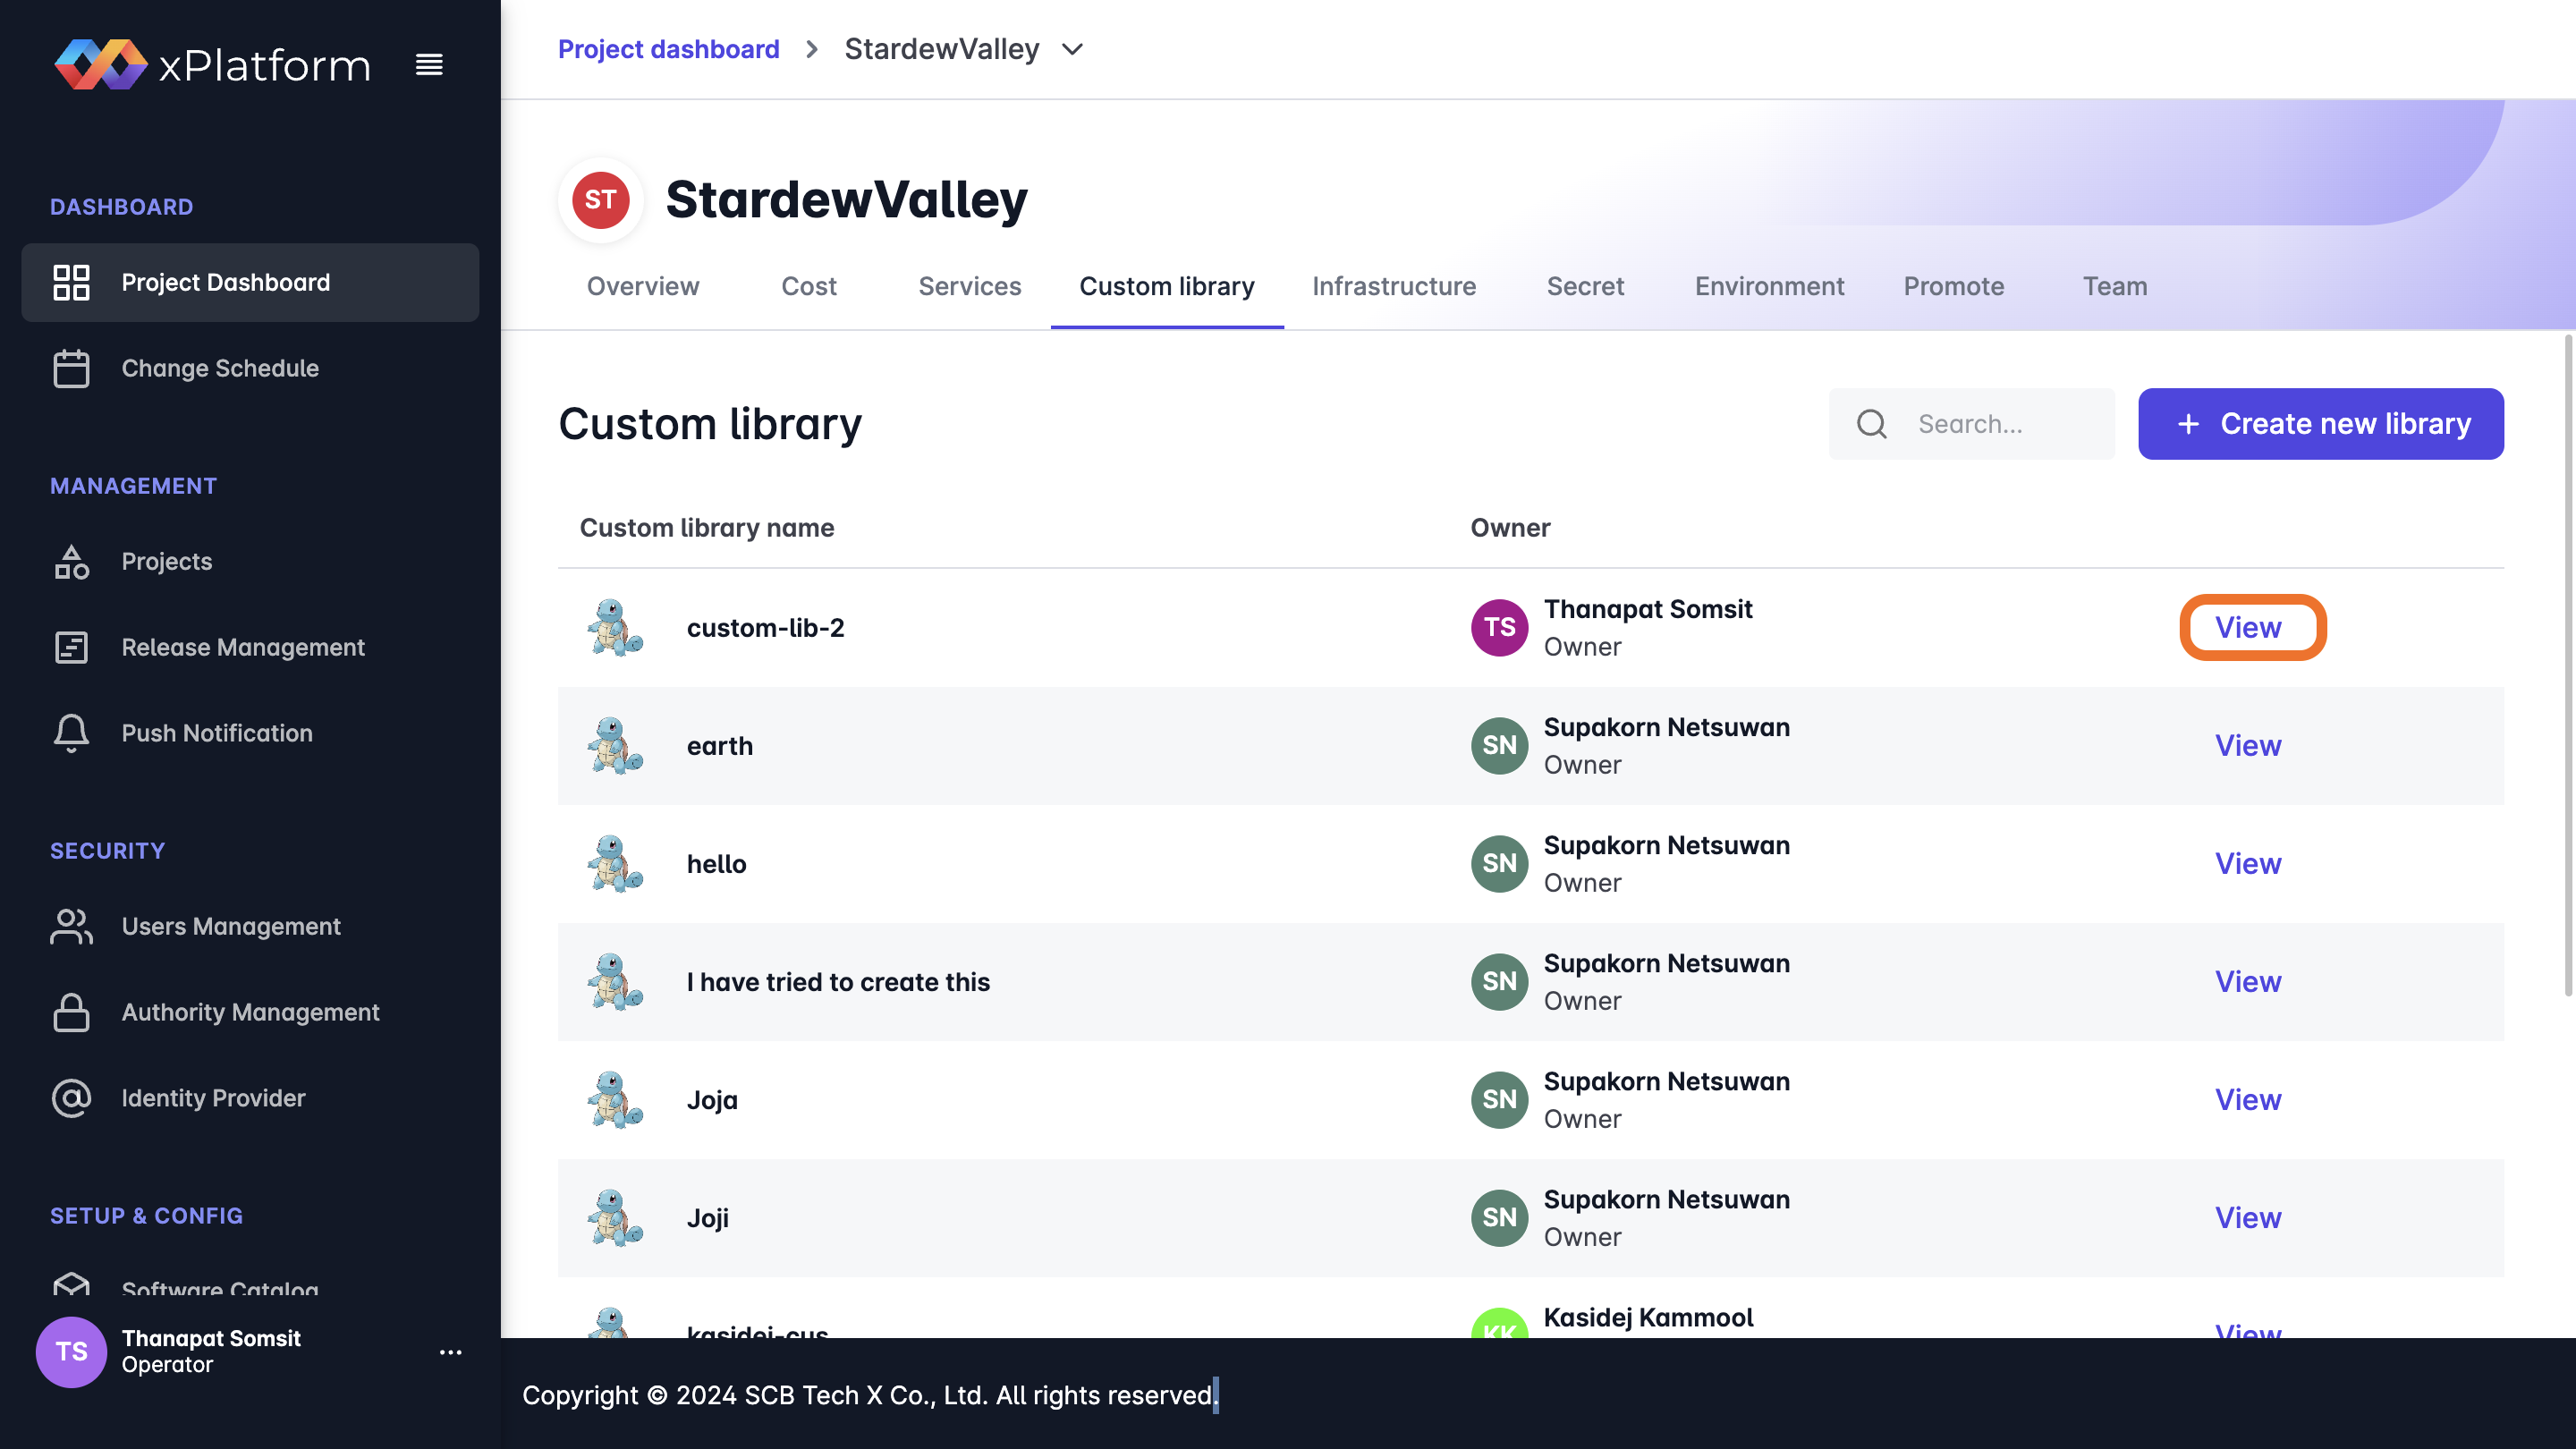
\includegraphics[width=\linewidth]{resources/pages/custom-library/create-library/1.png}

    \vspace{1in}

    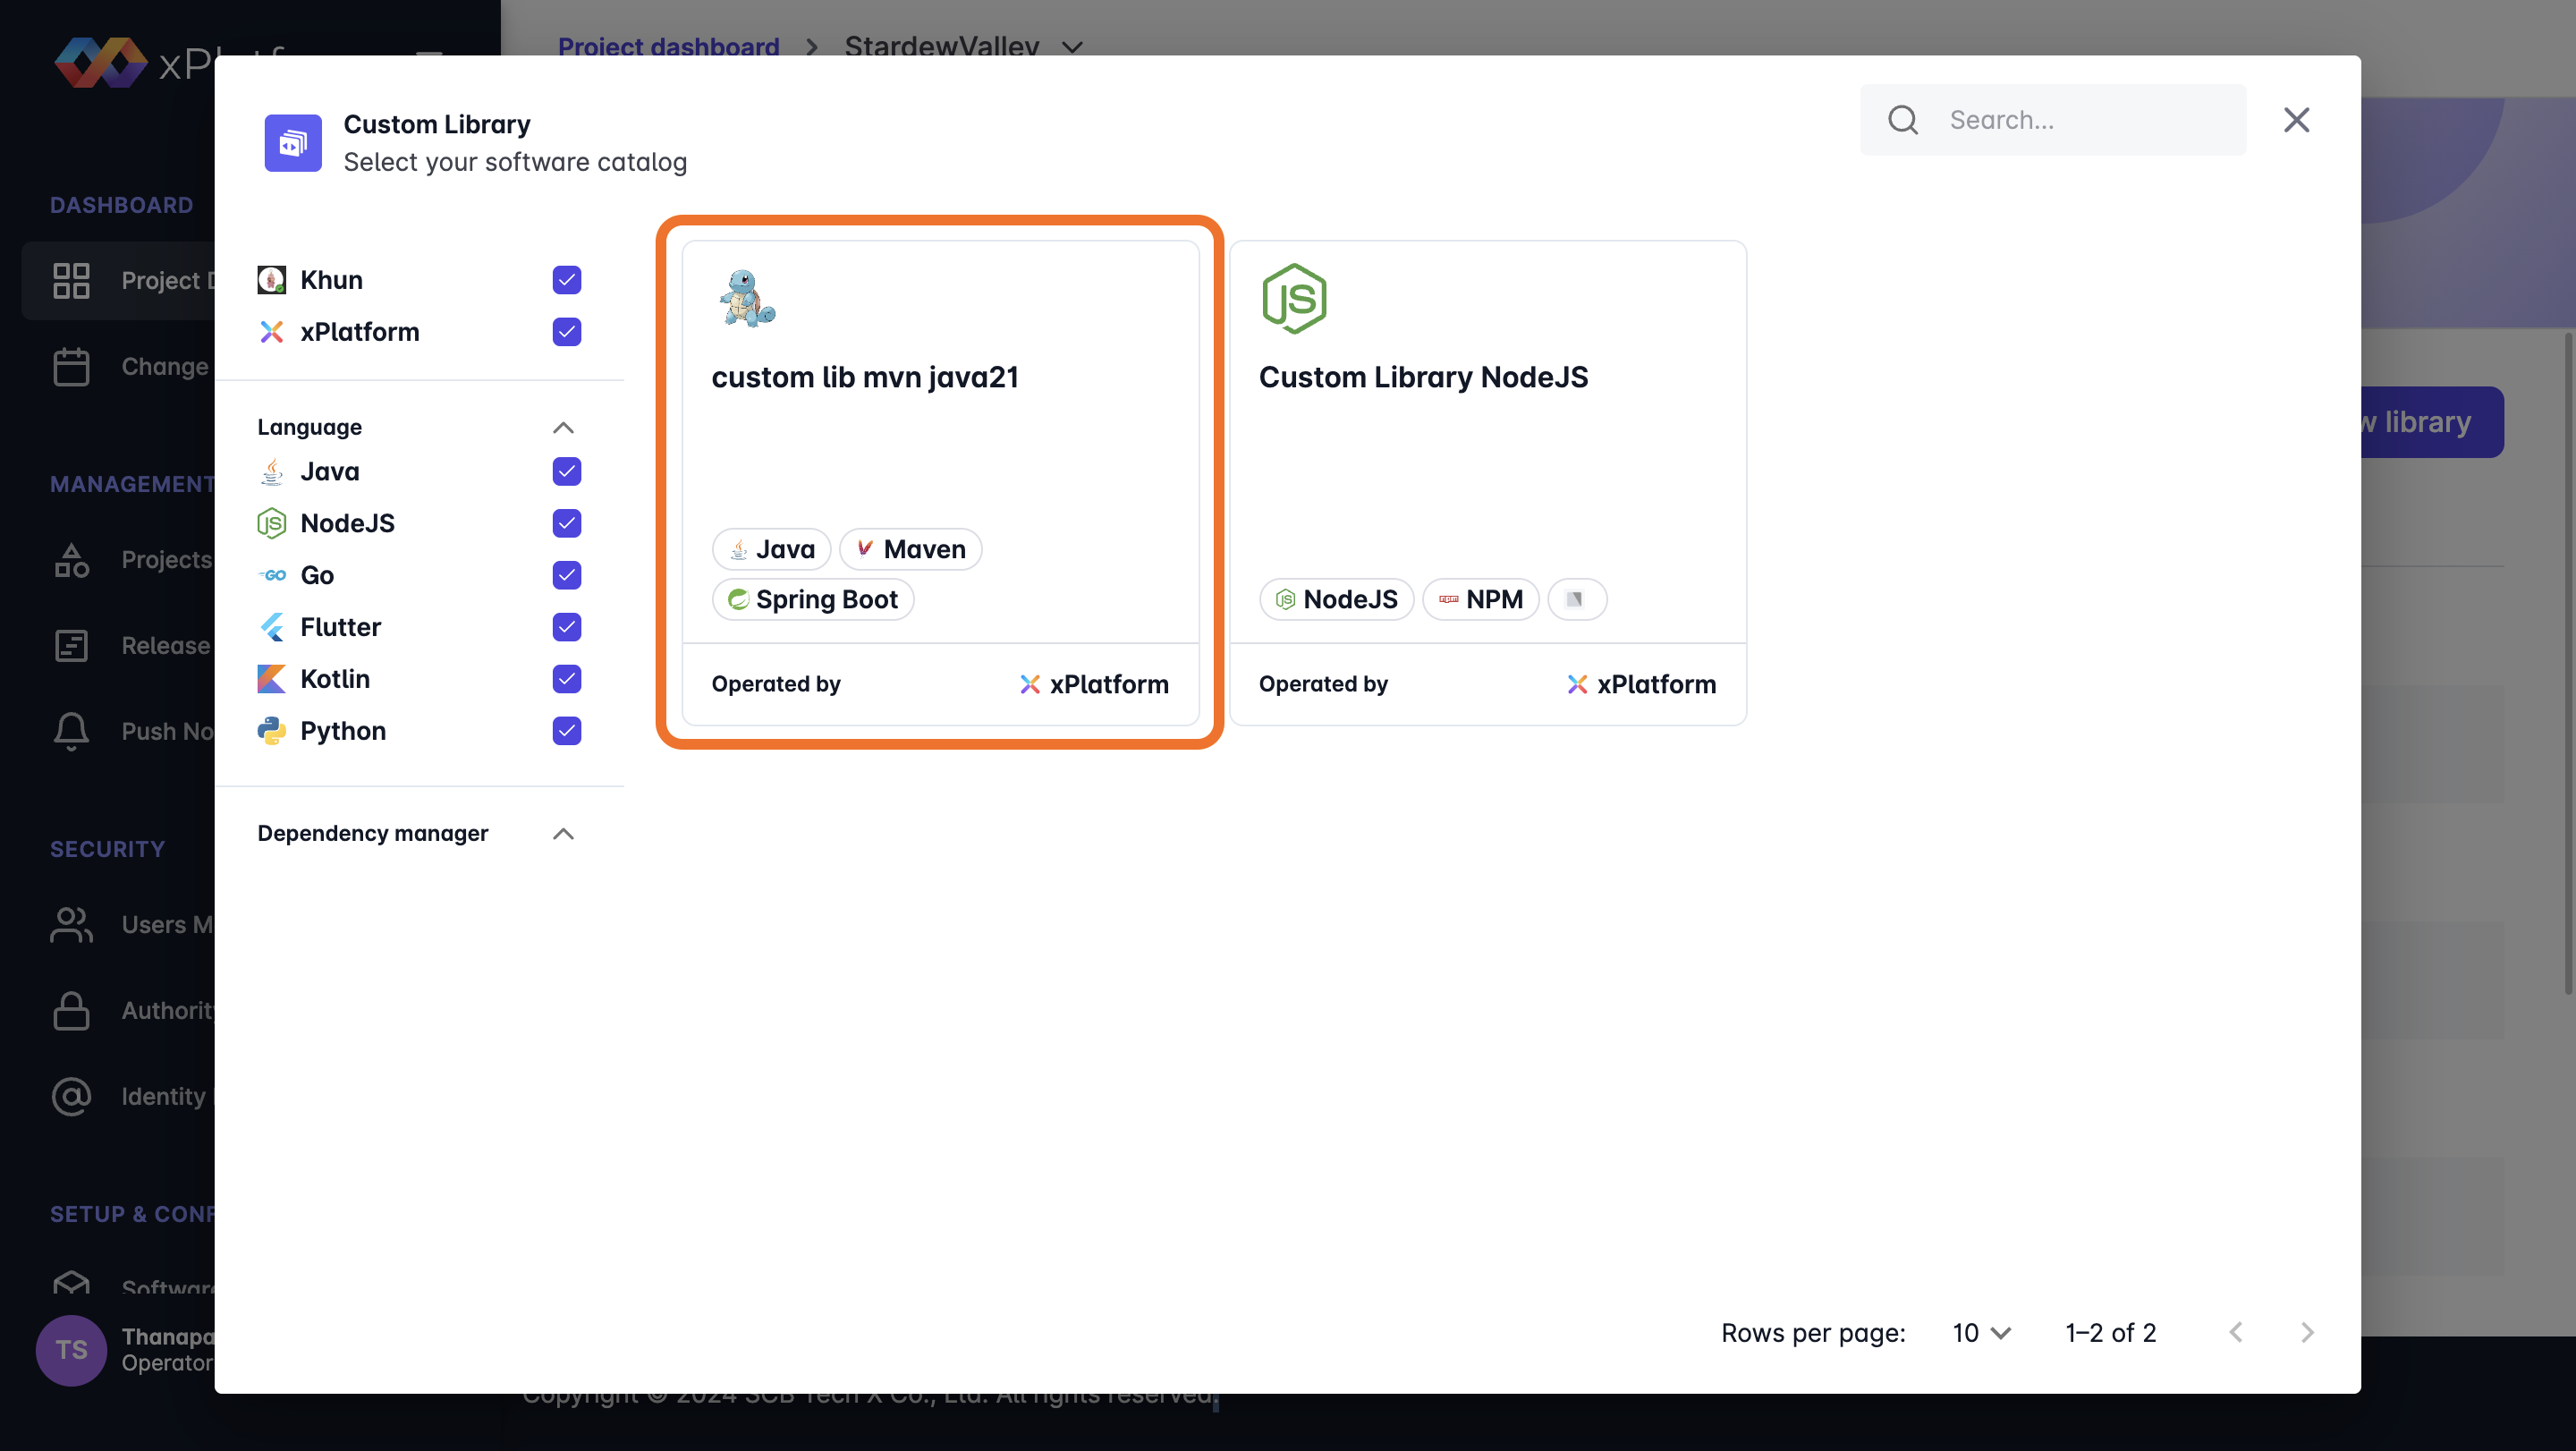
\includegraphics[width=\linewidth]{resources/pages/custom-library/create-library/2.png}
\end{center}
\begin{center}
    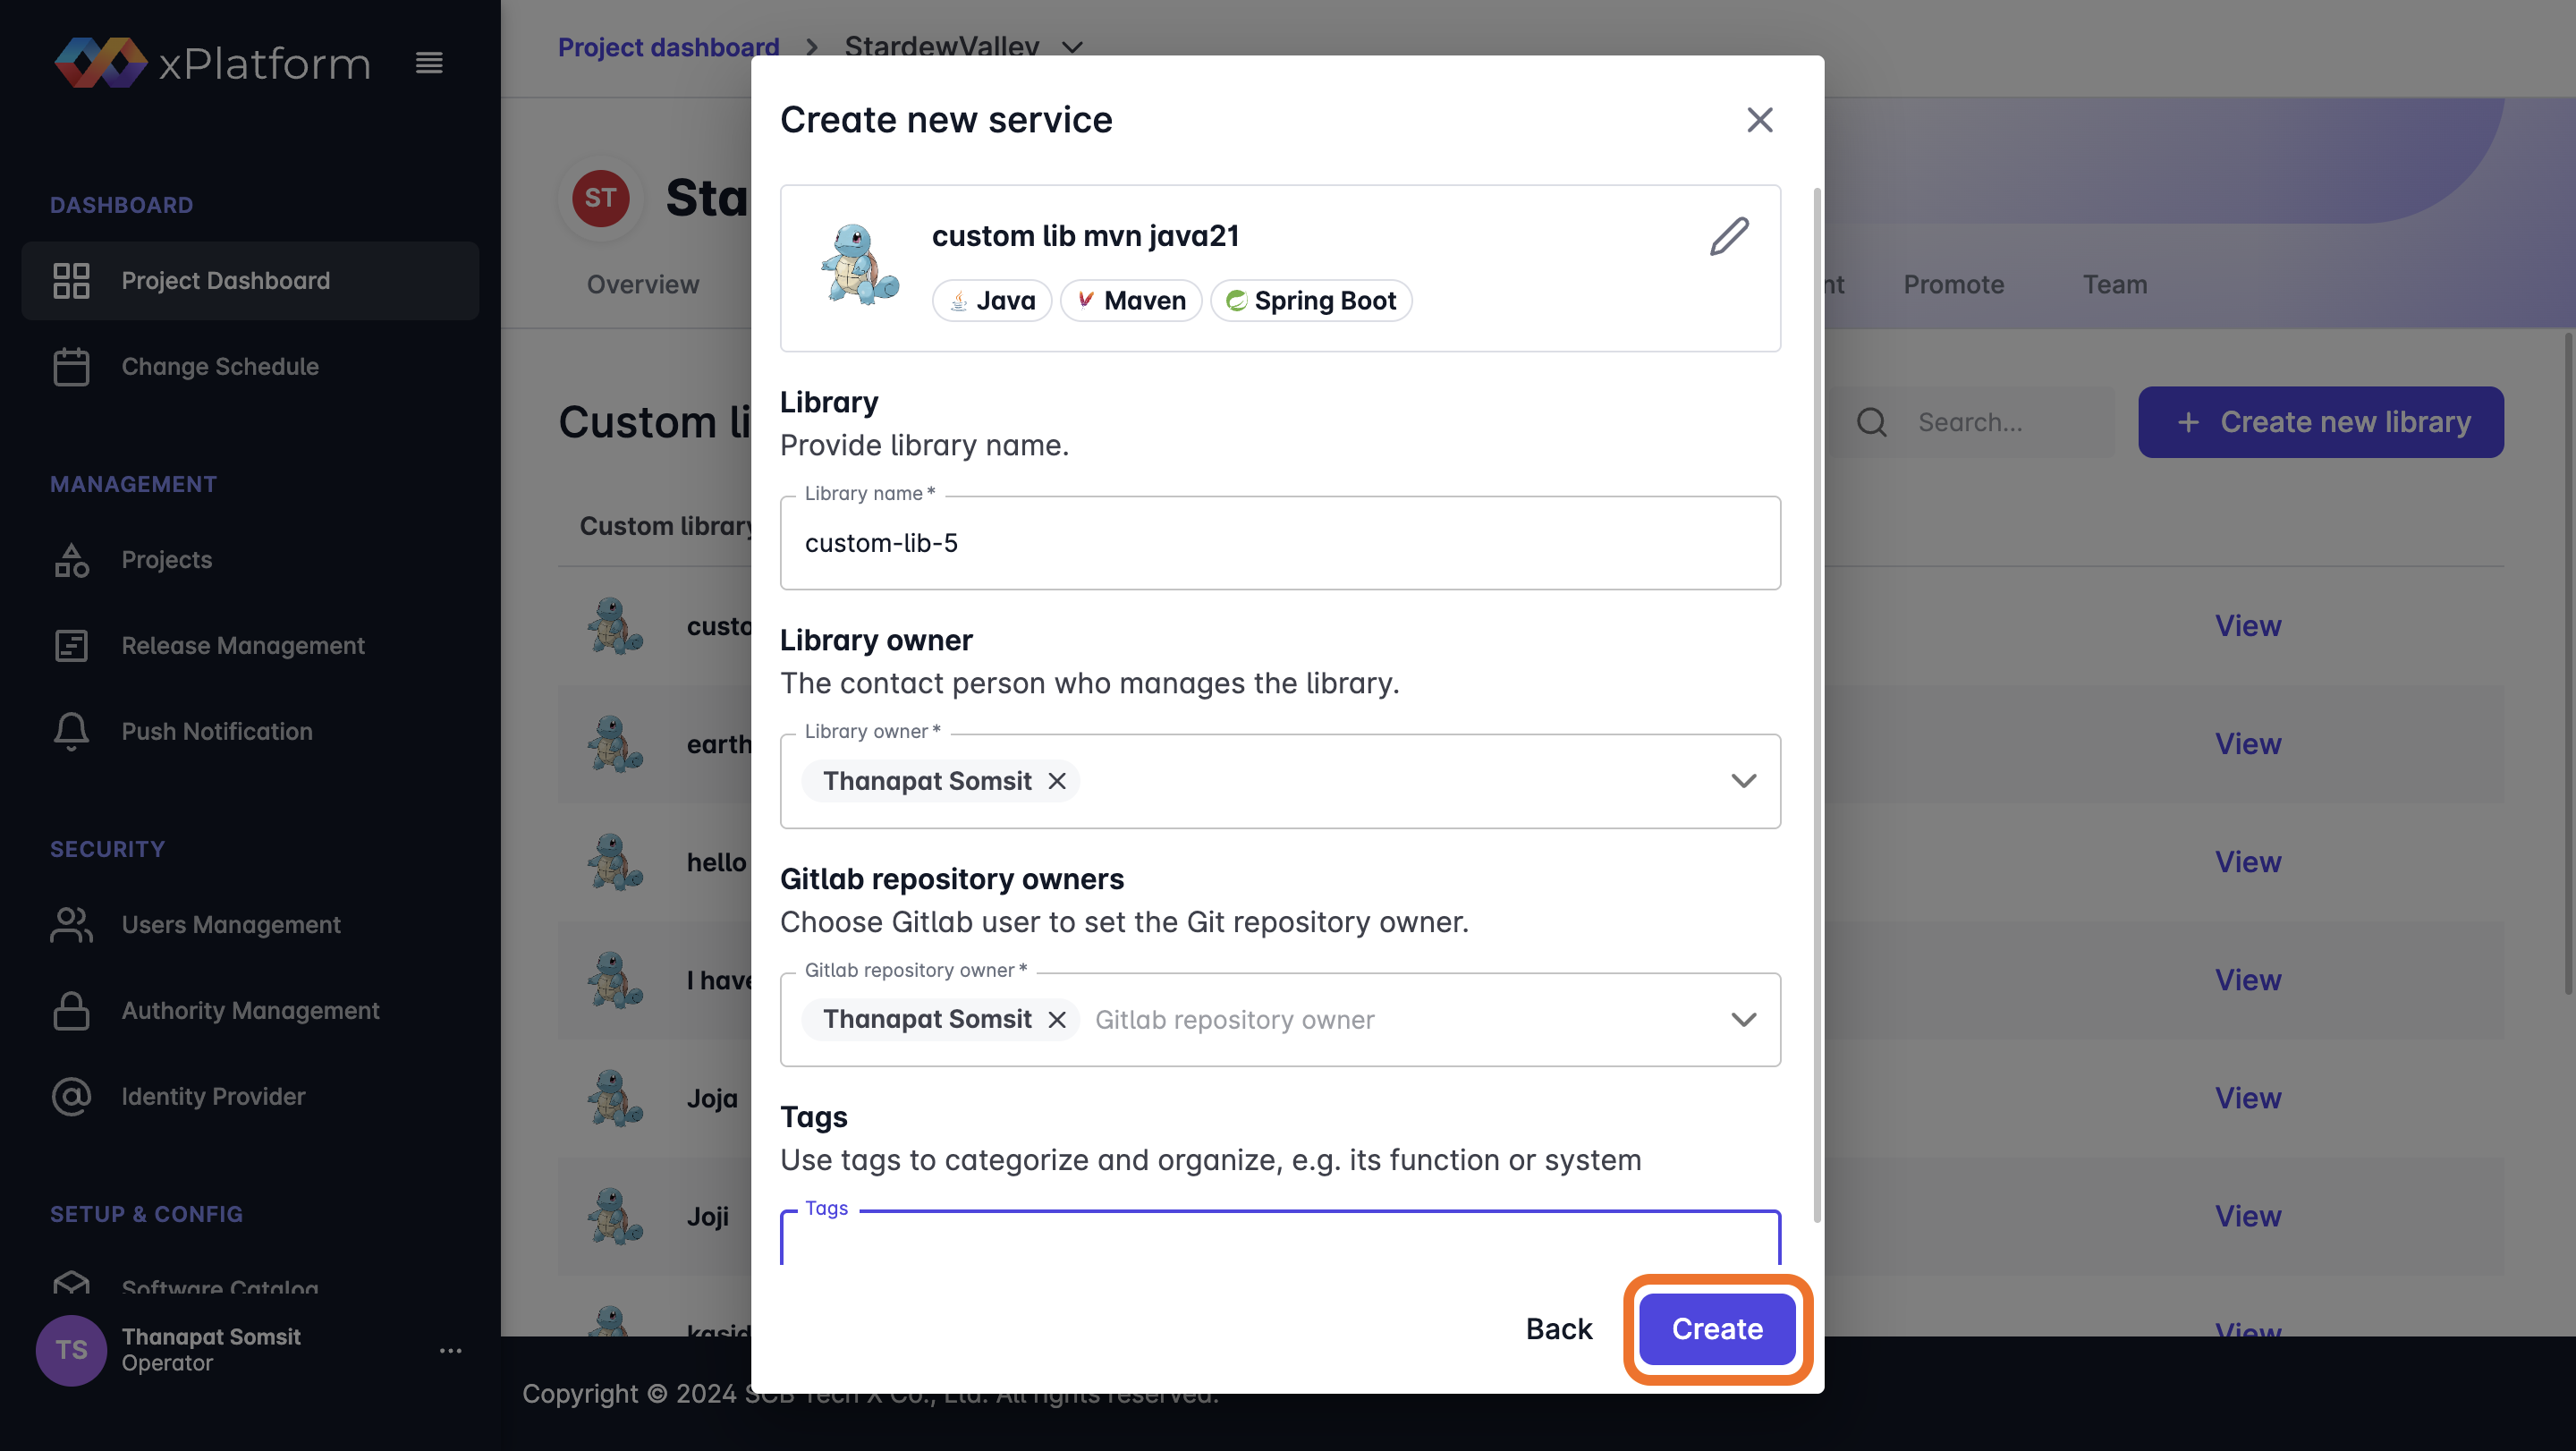
\includegraphics[width=\linewidth]{resources/pages/custom-library/create-library/3.png}

    \vspace{1in}

    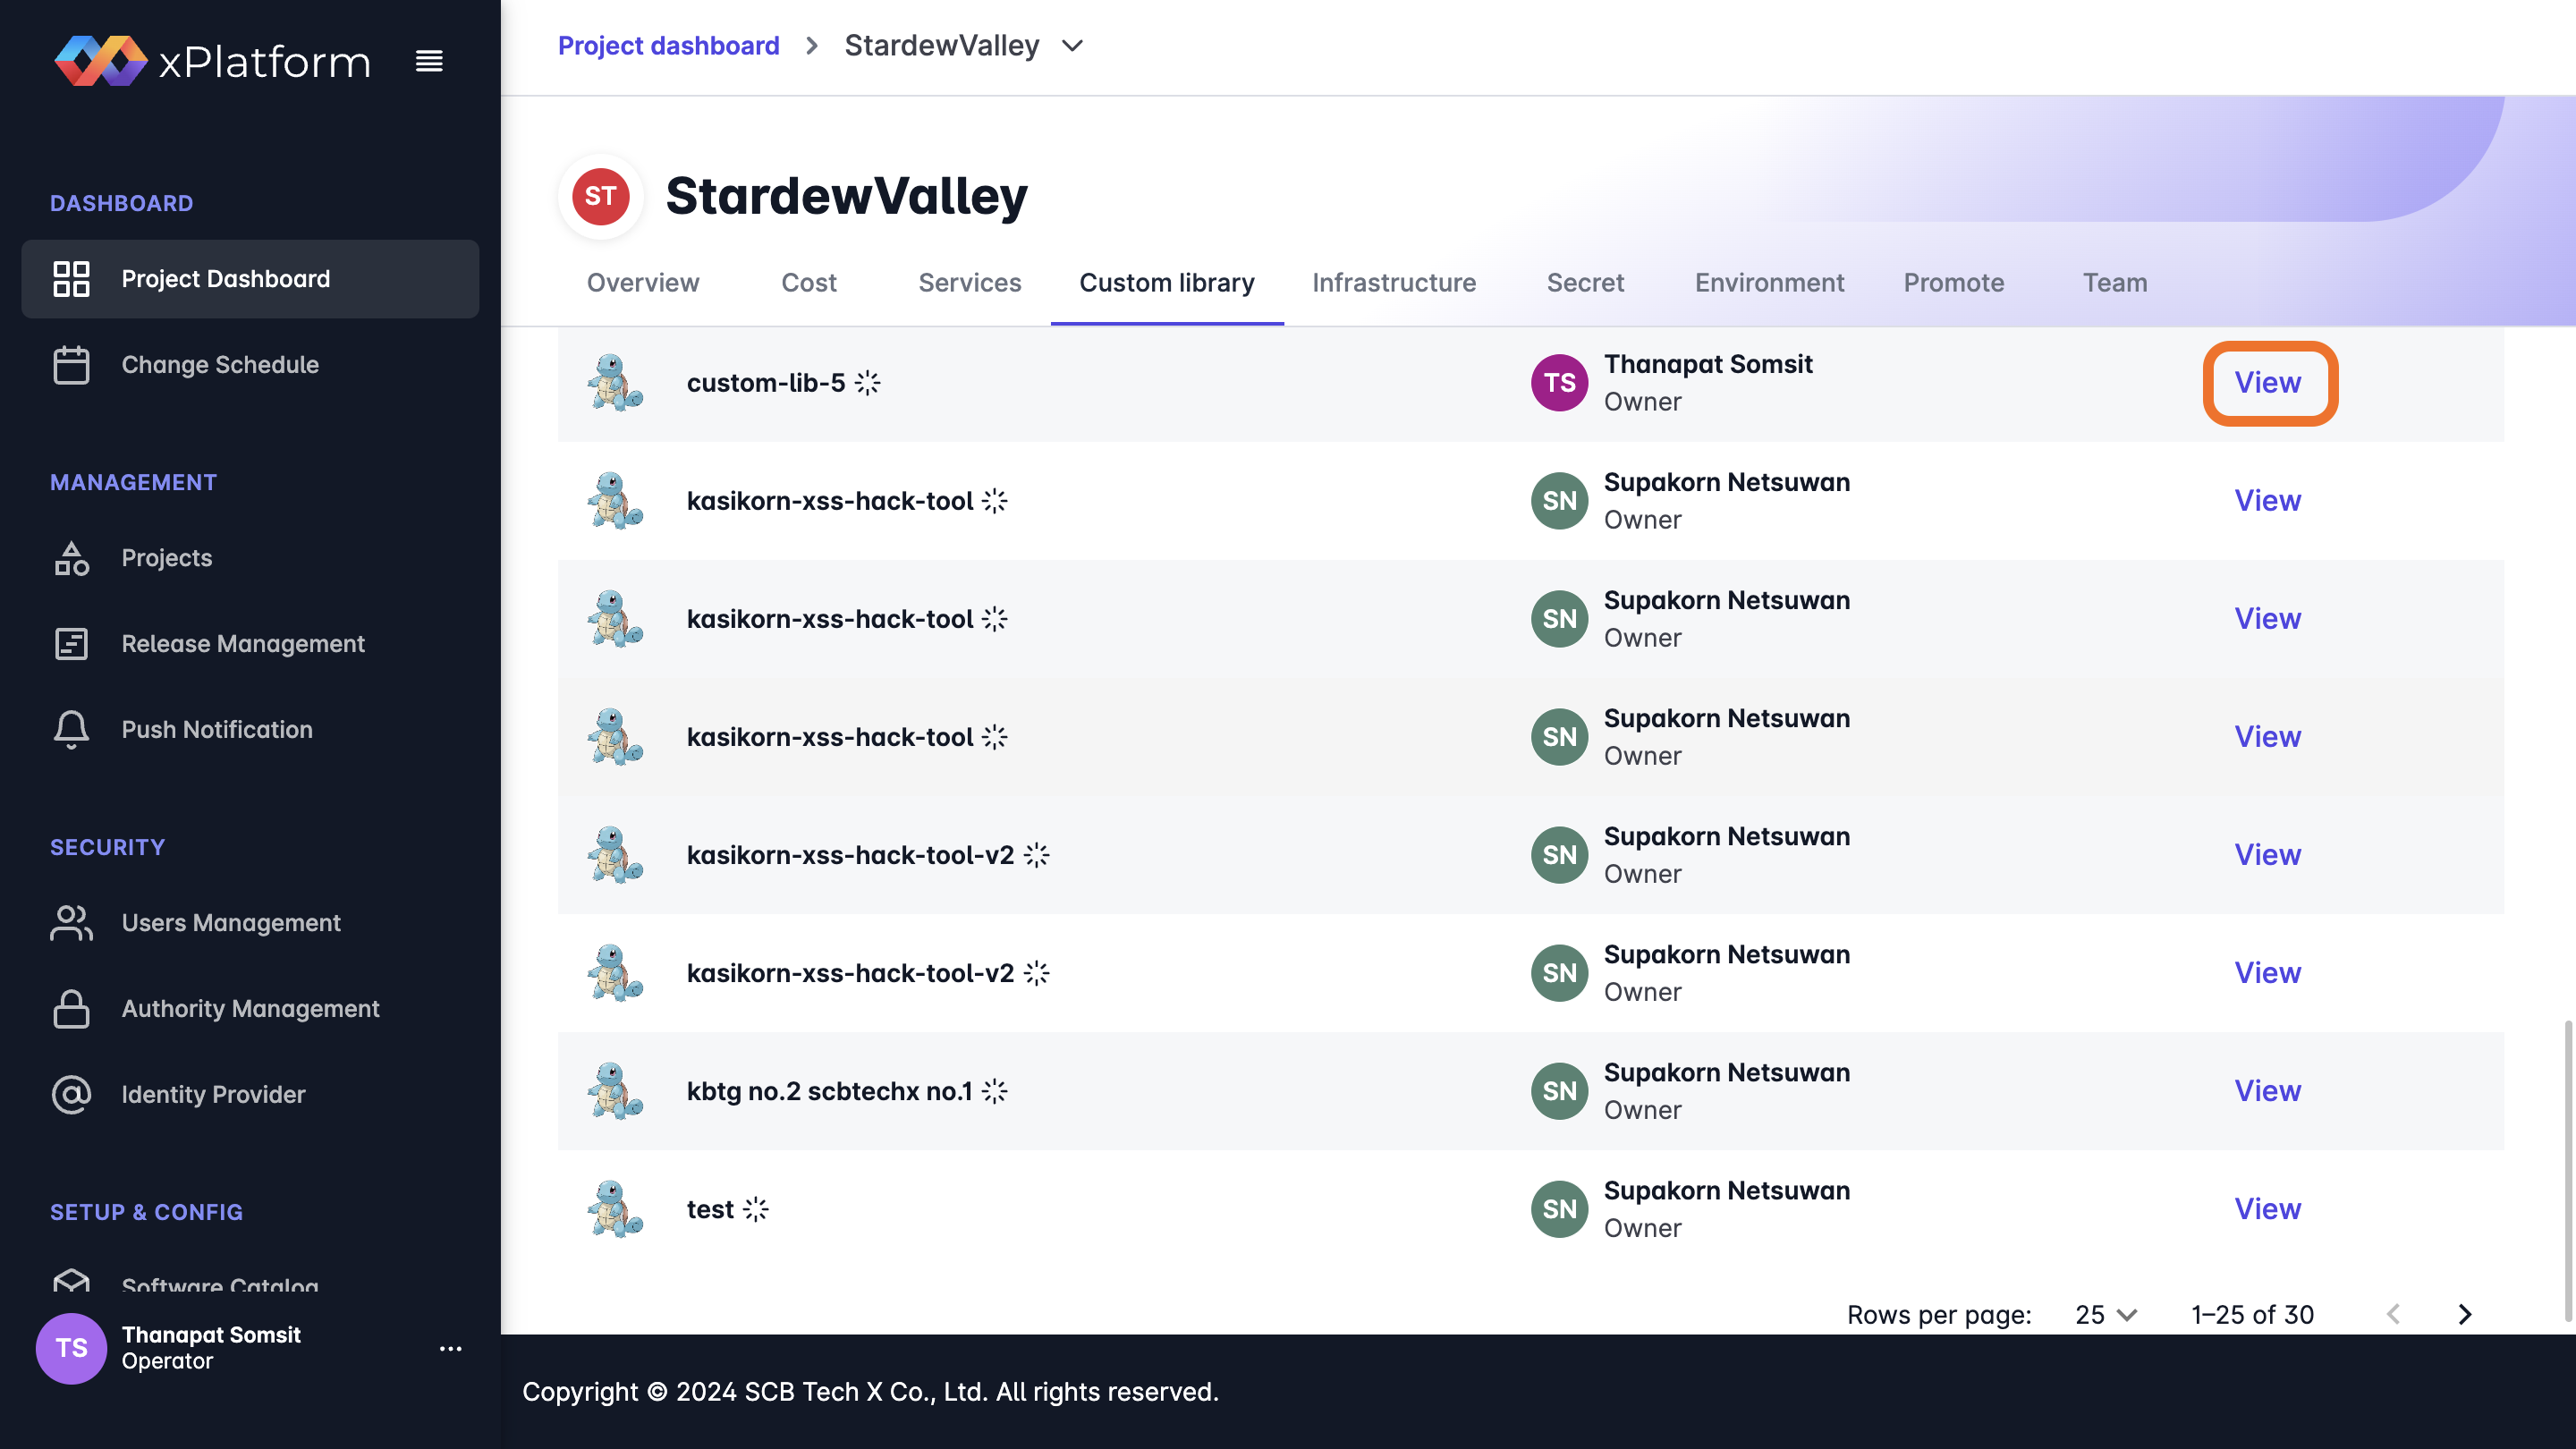
\includegraphics[width=\linewidth]{resources/pages/custom-library/create-library/4.png}
\end{center}

\begin{figure}[H]
    \begin{center}
        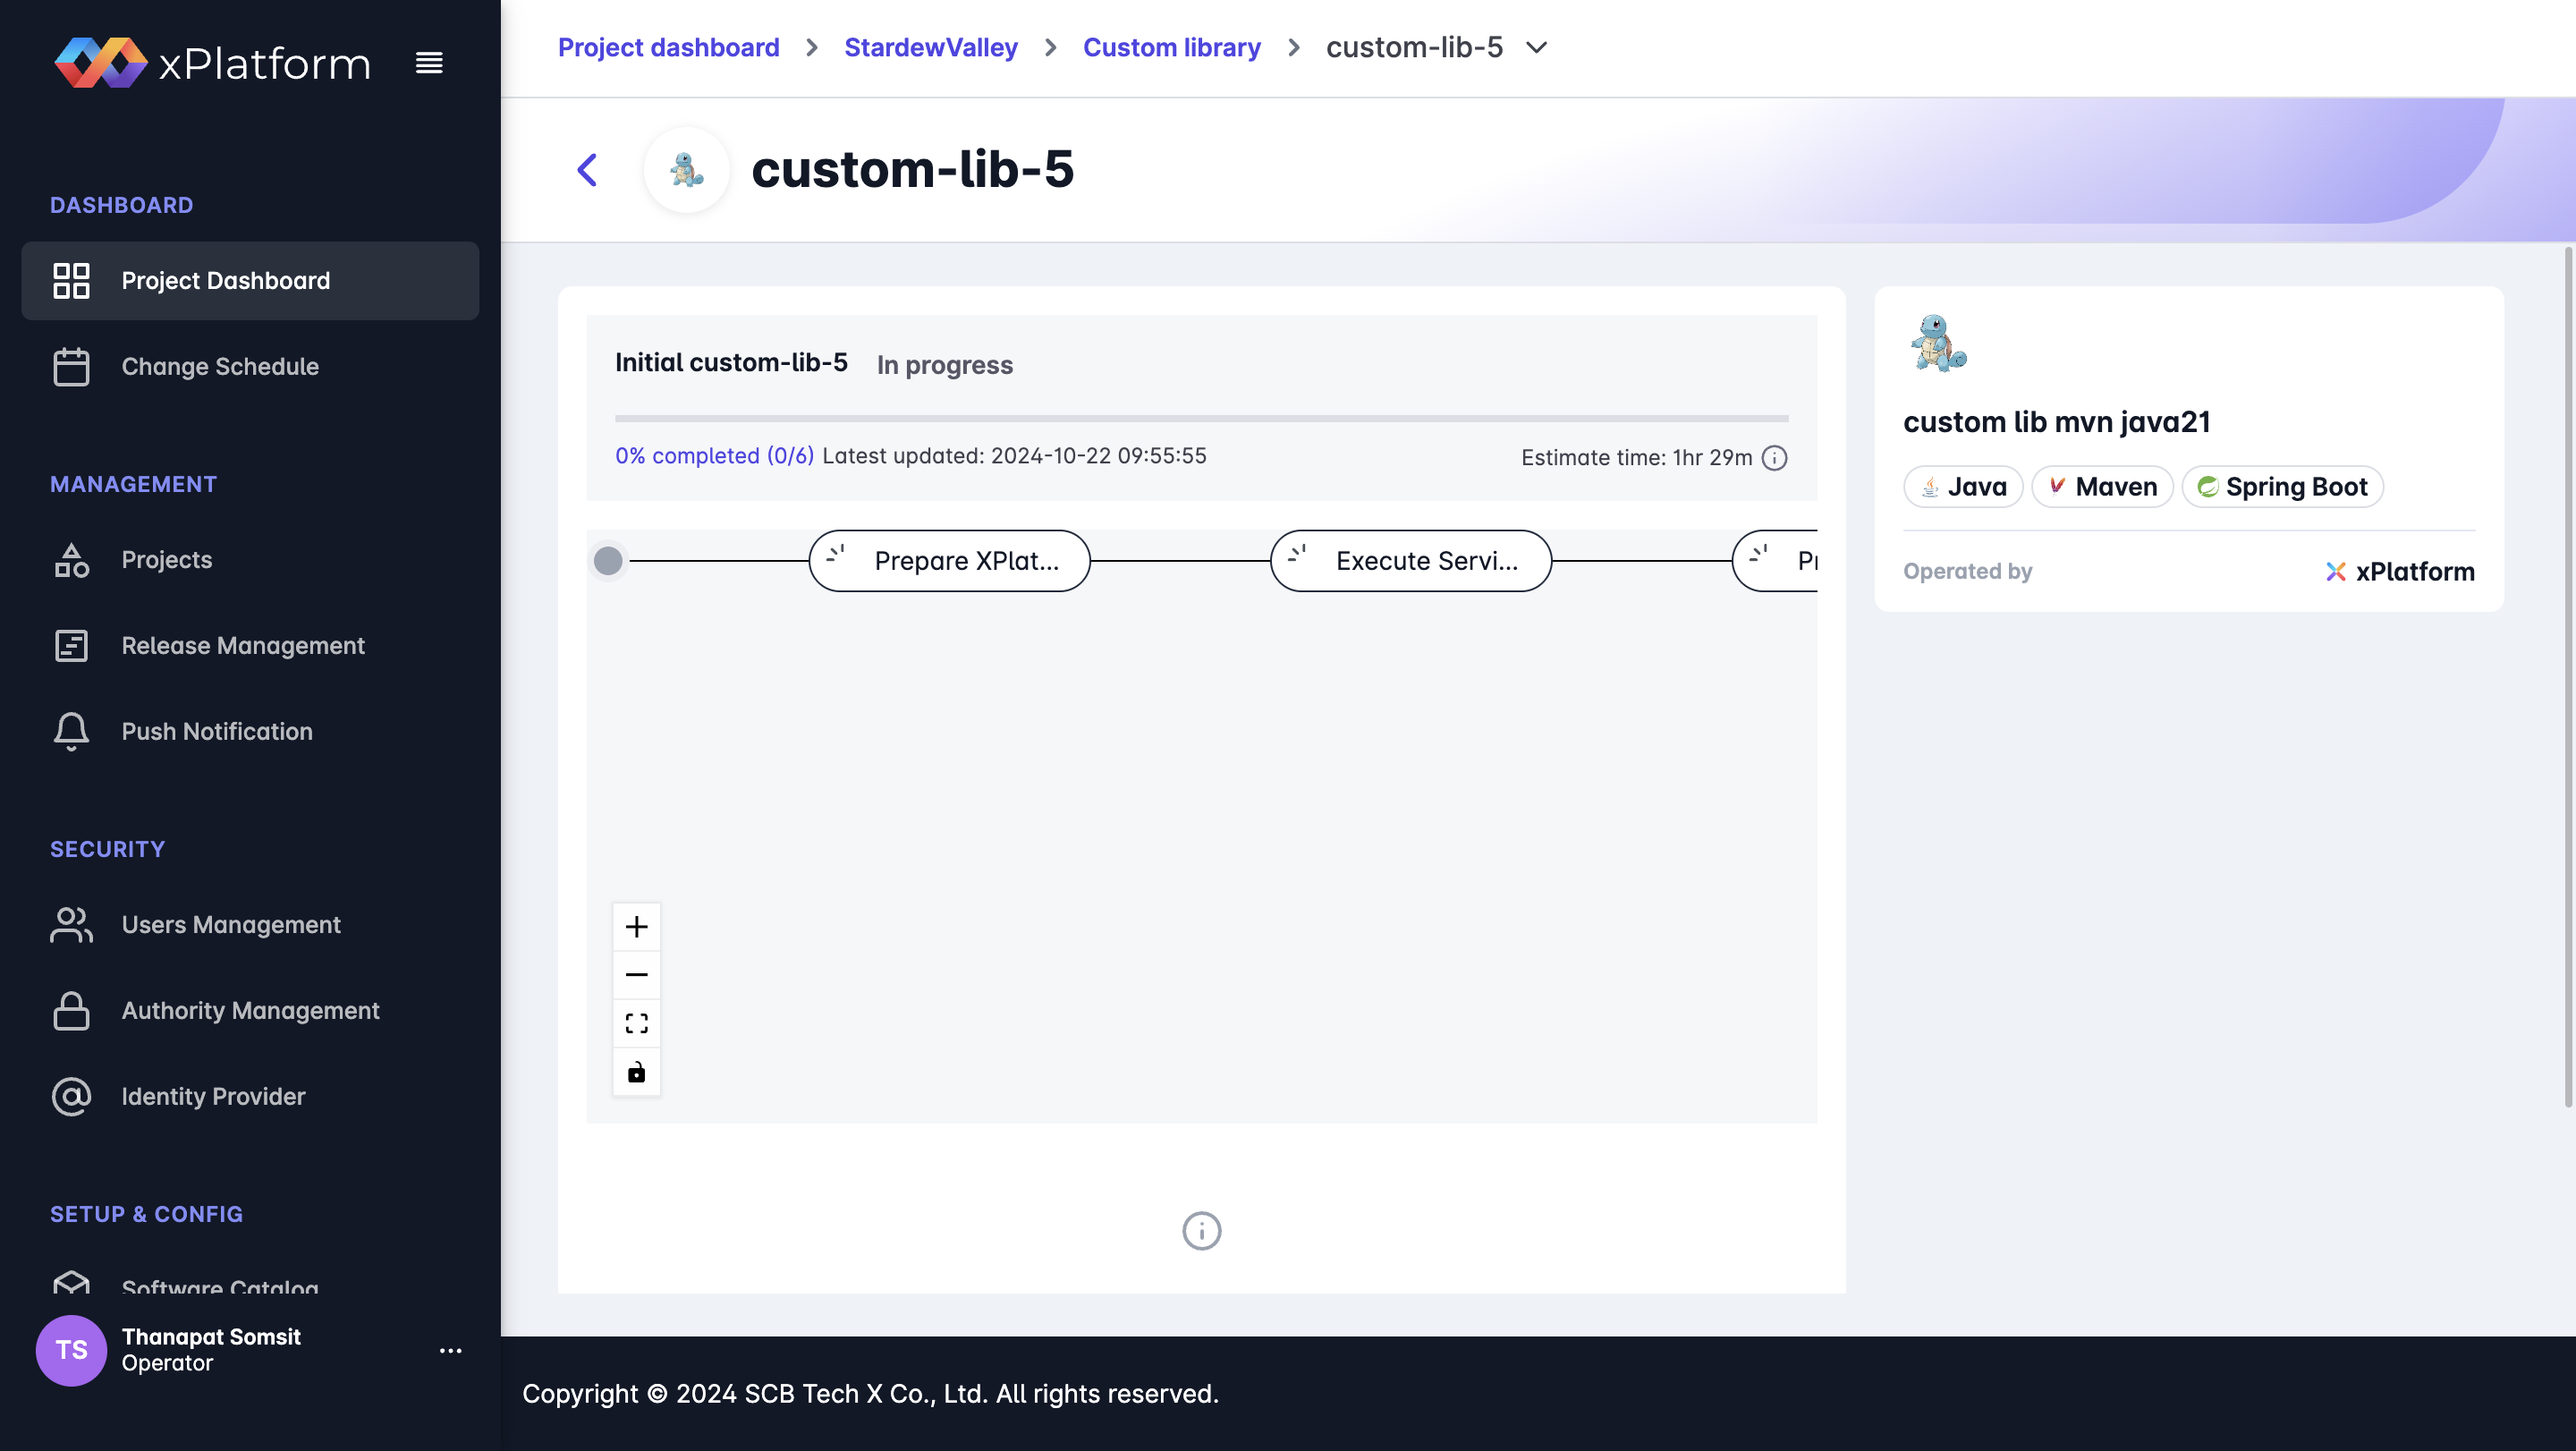
\includegraphics[width=\linewidth]{resources/pages/custom-library/create-library/5.png}
    
        \vspace{1in}
    
        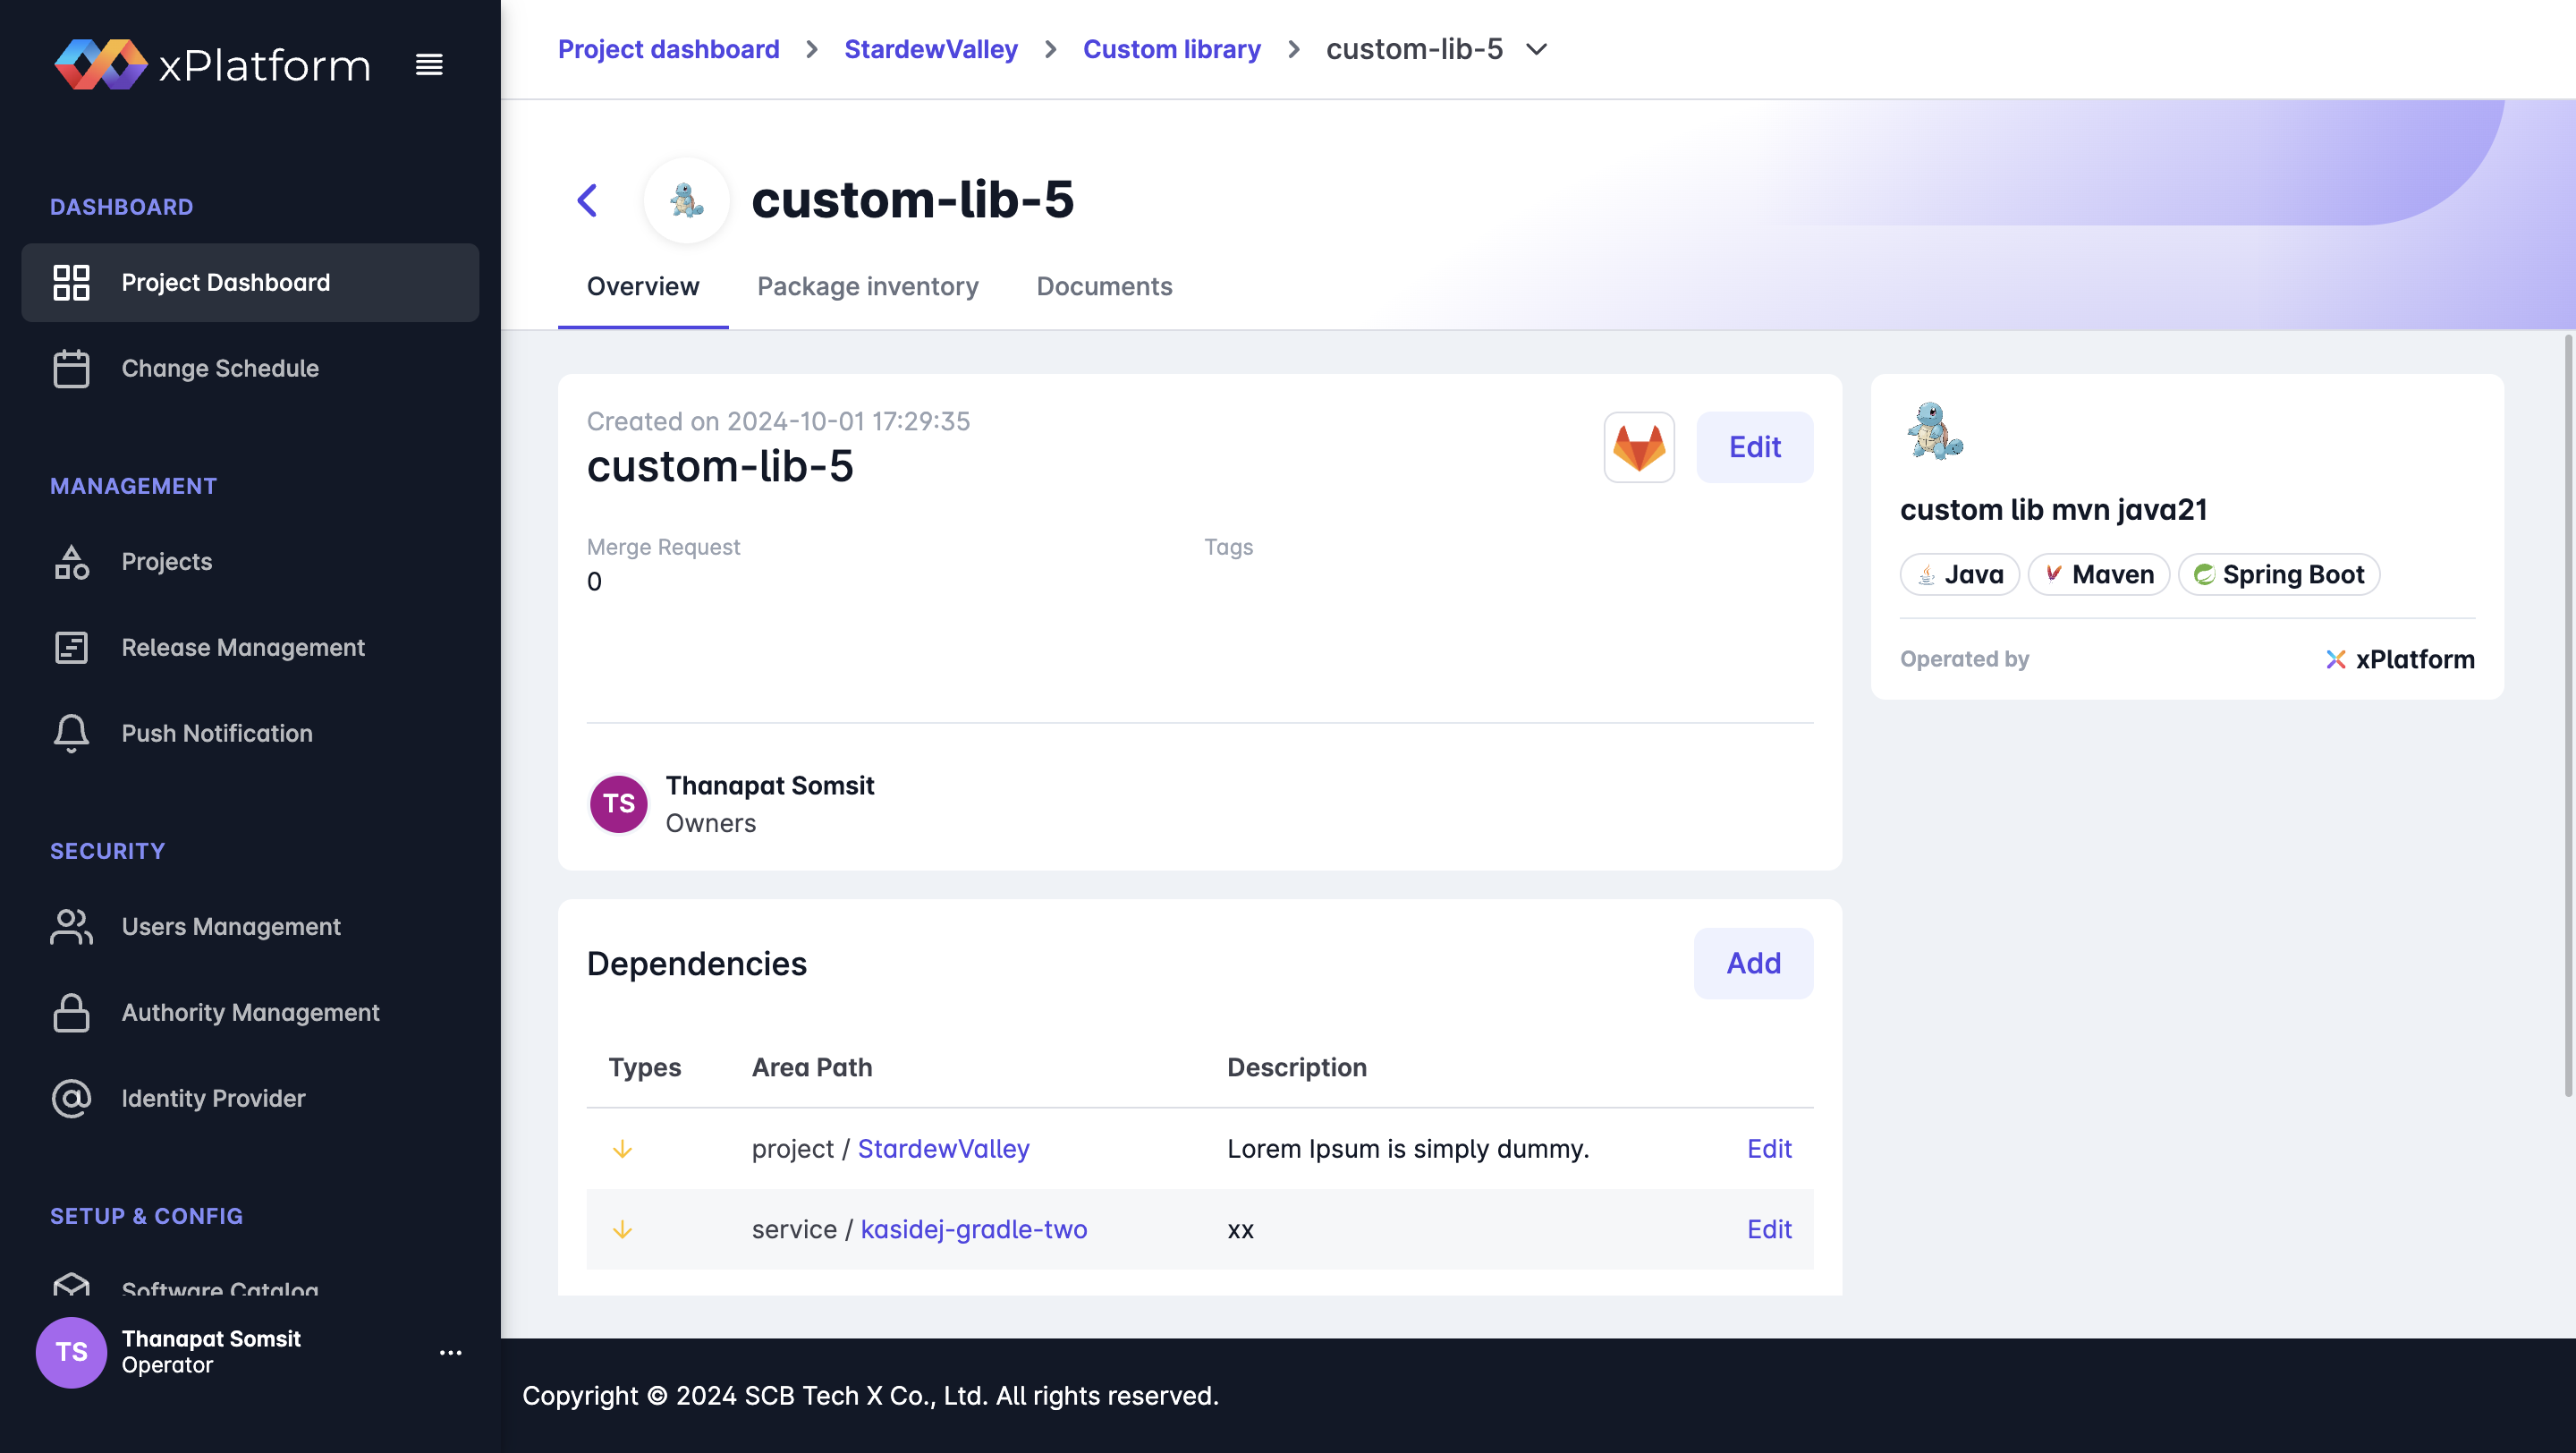
\includegraphics[width=\linewidth]{resources/pages/custom-library/create-library/6.png}
    \end{center}
    \caption[การสร้าง Custom Library]{การสร้าง Custom Library}
  \label{fig:create-library}
\end{figure}

\newpage
\subsection{การอัพเดตเวอร์ชัน Custom Library}
\begin{center}
    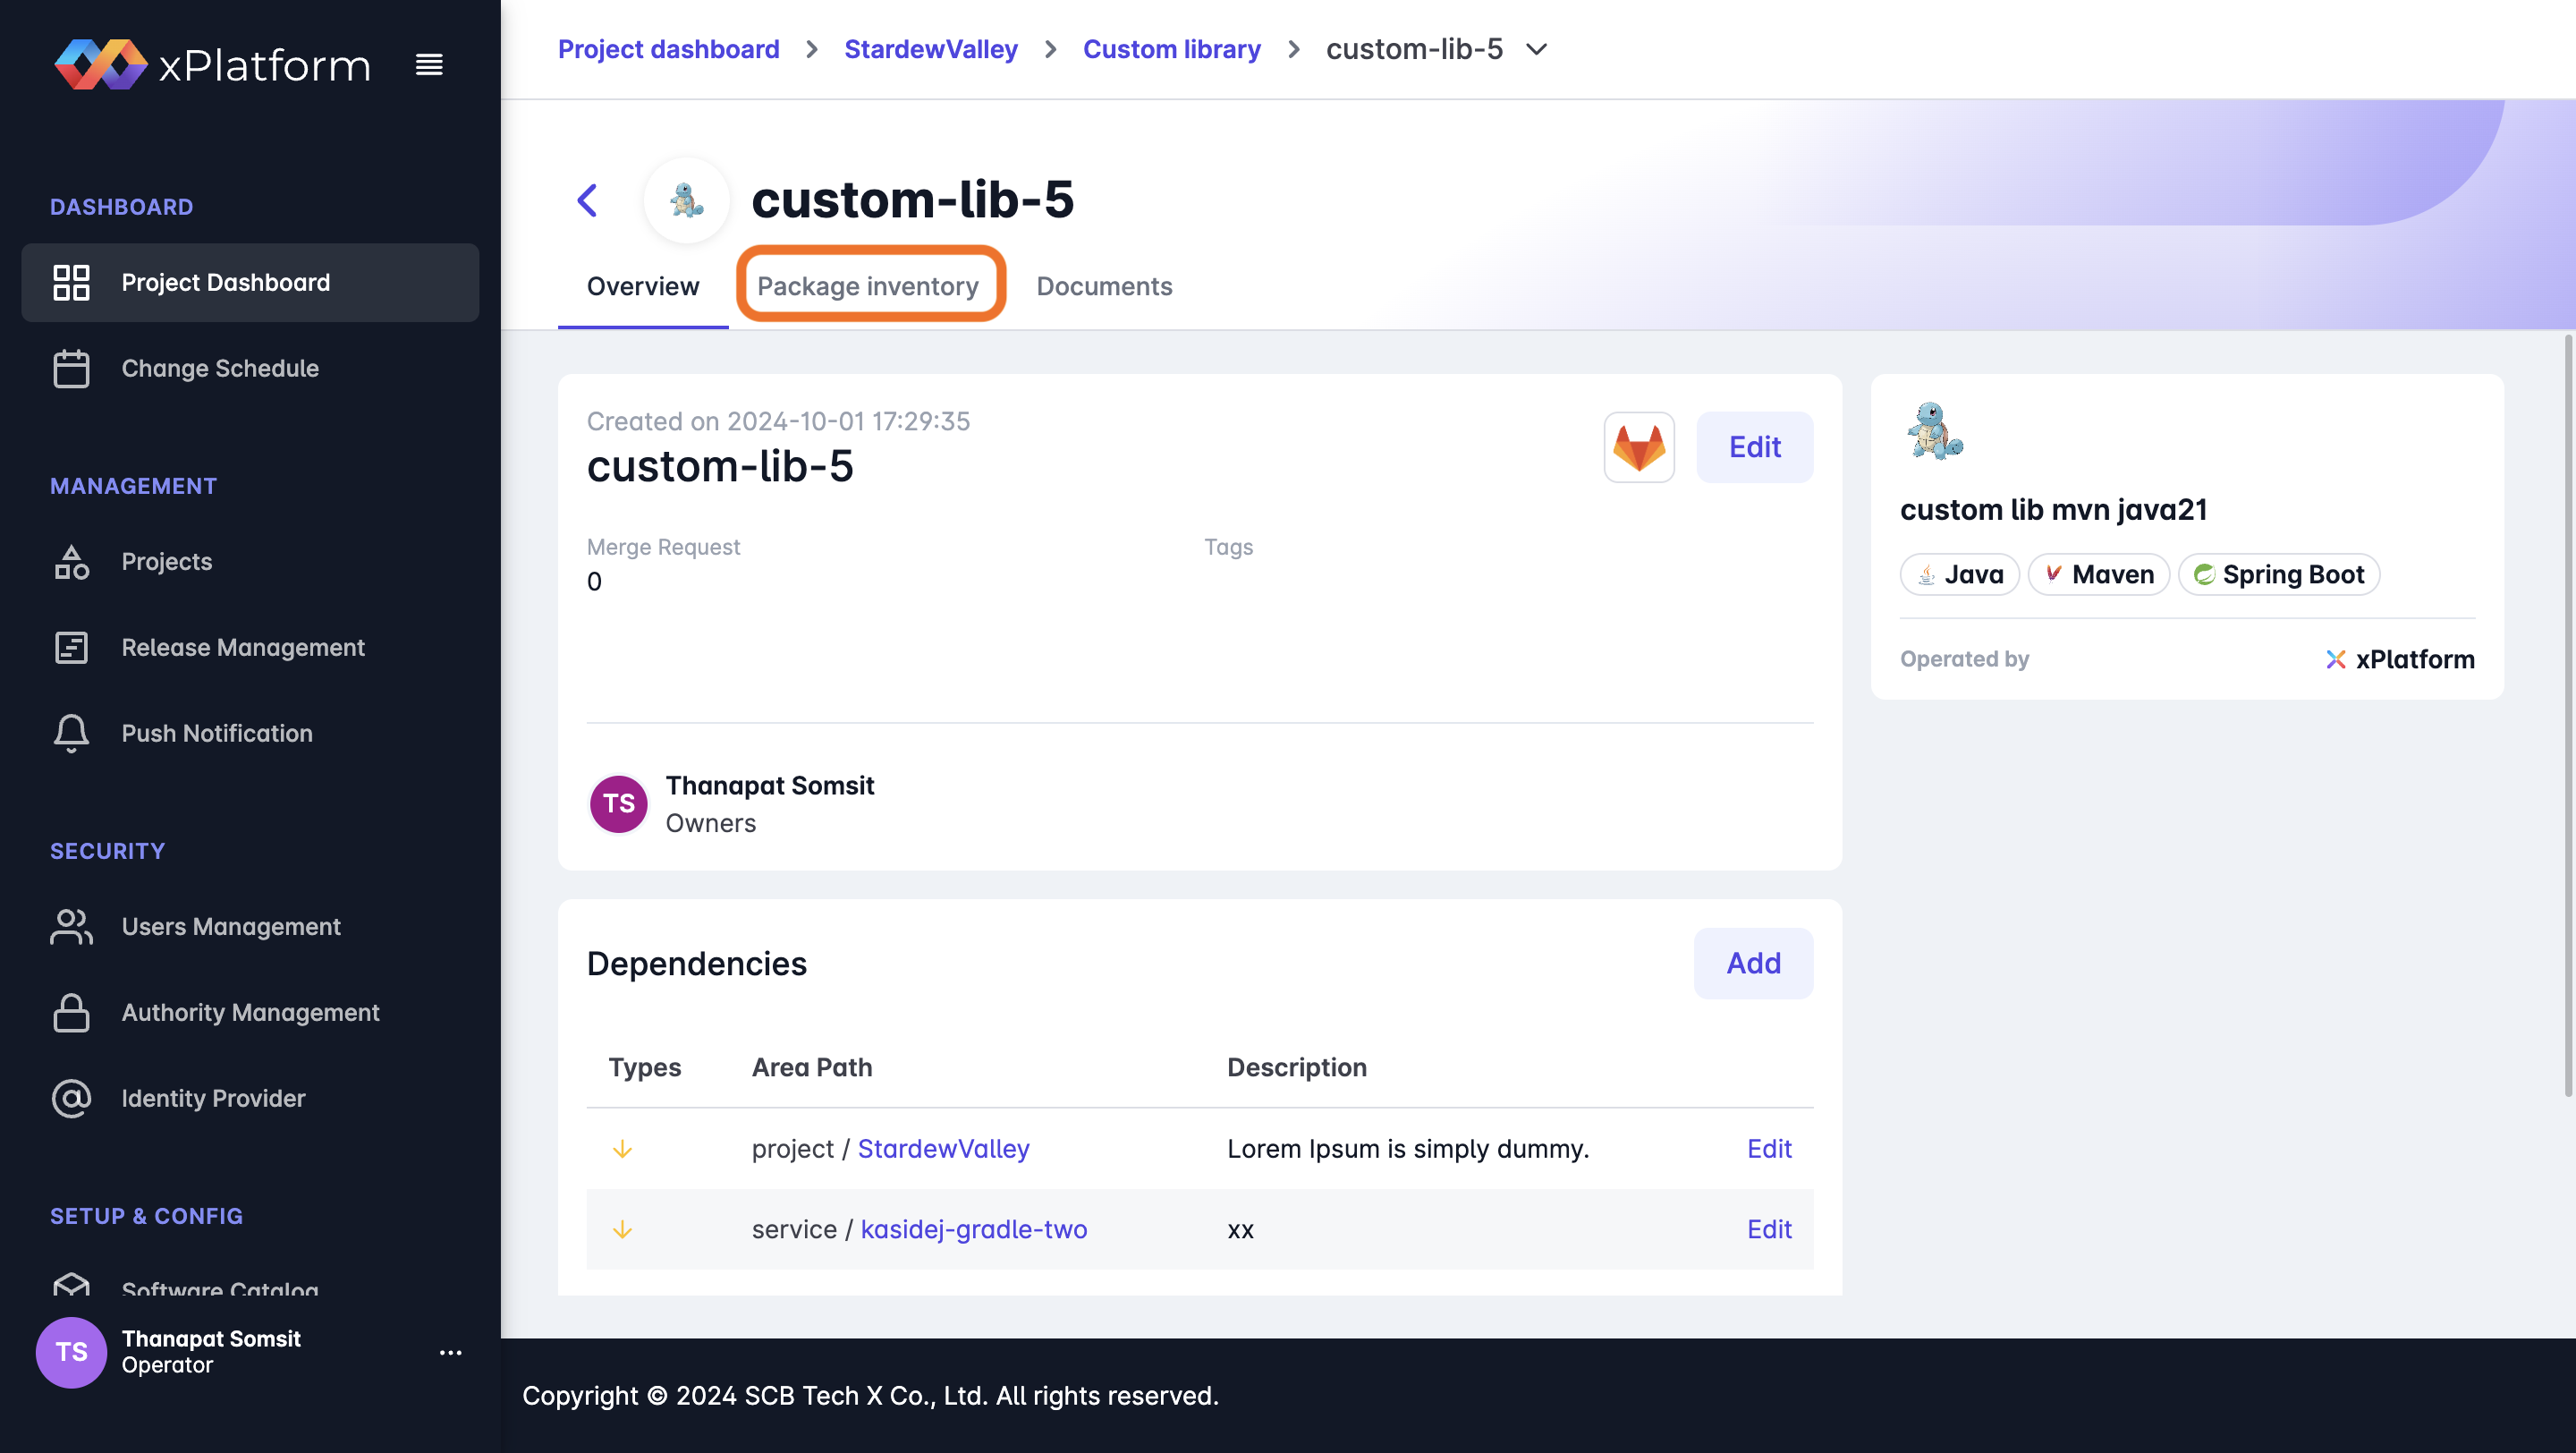
\includegraphics[width=\linewidth]{resources/pages/custom-library/update-library/6.png}

    \vspace{1in}

    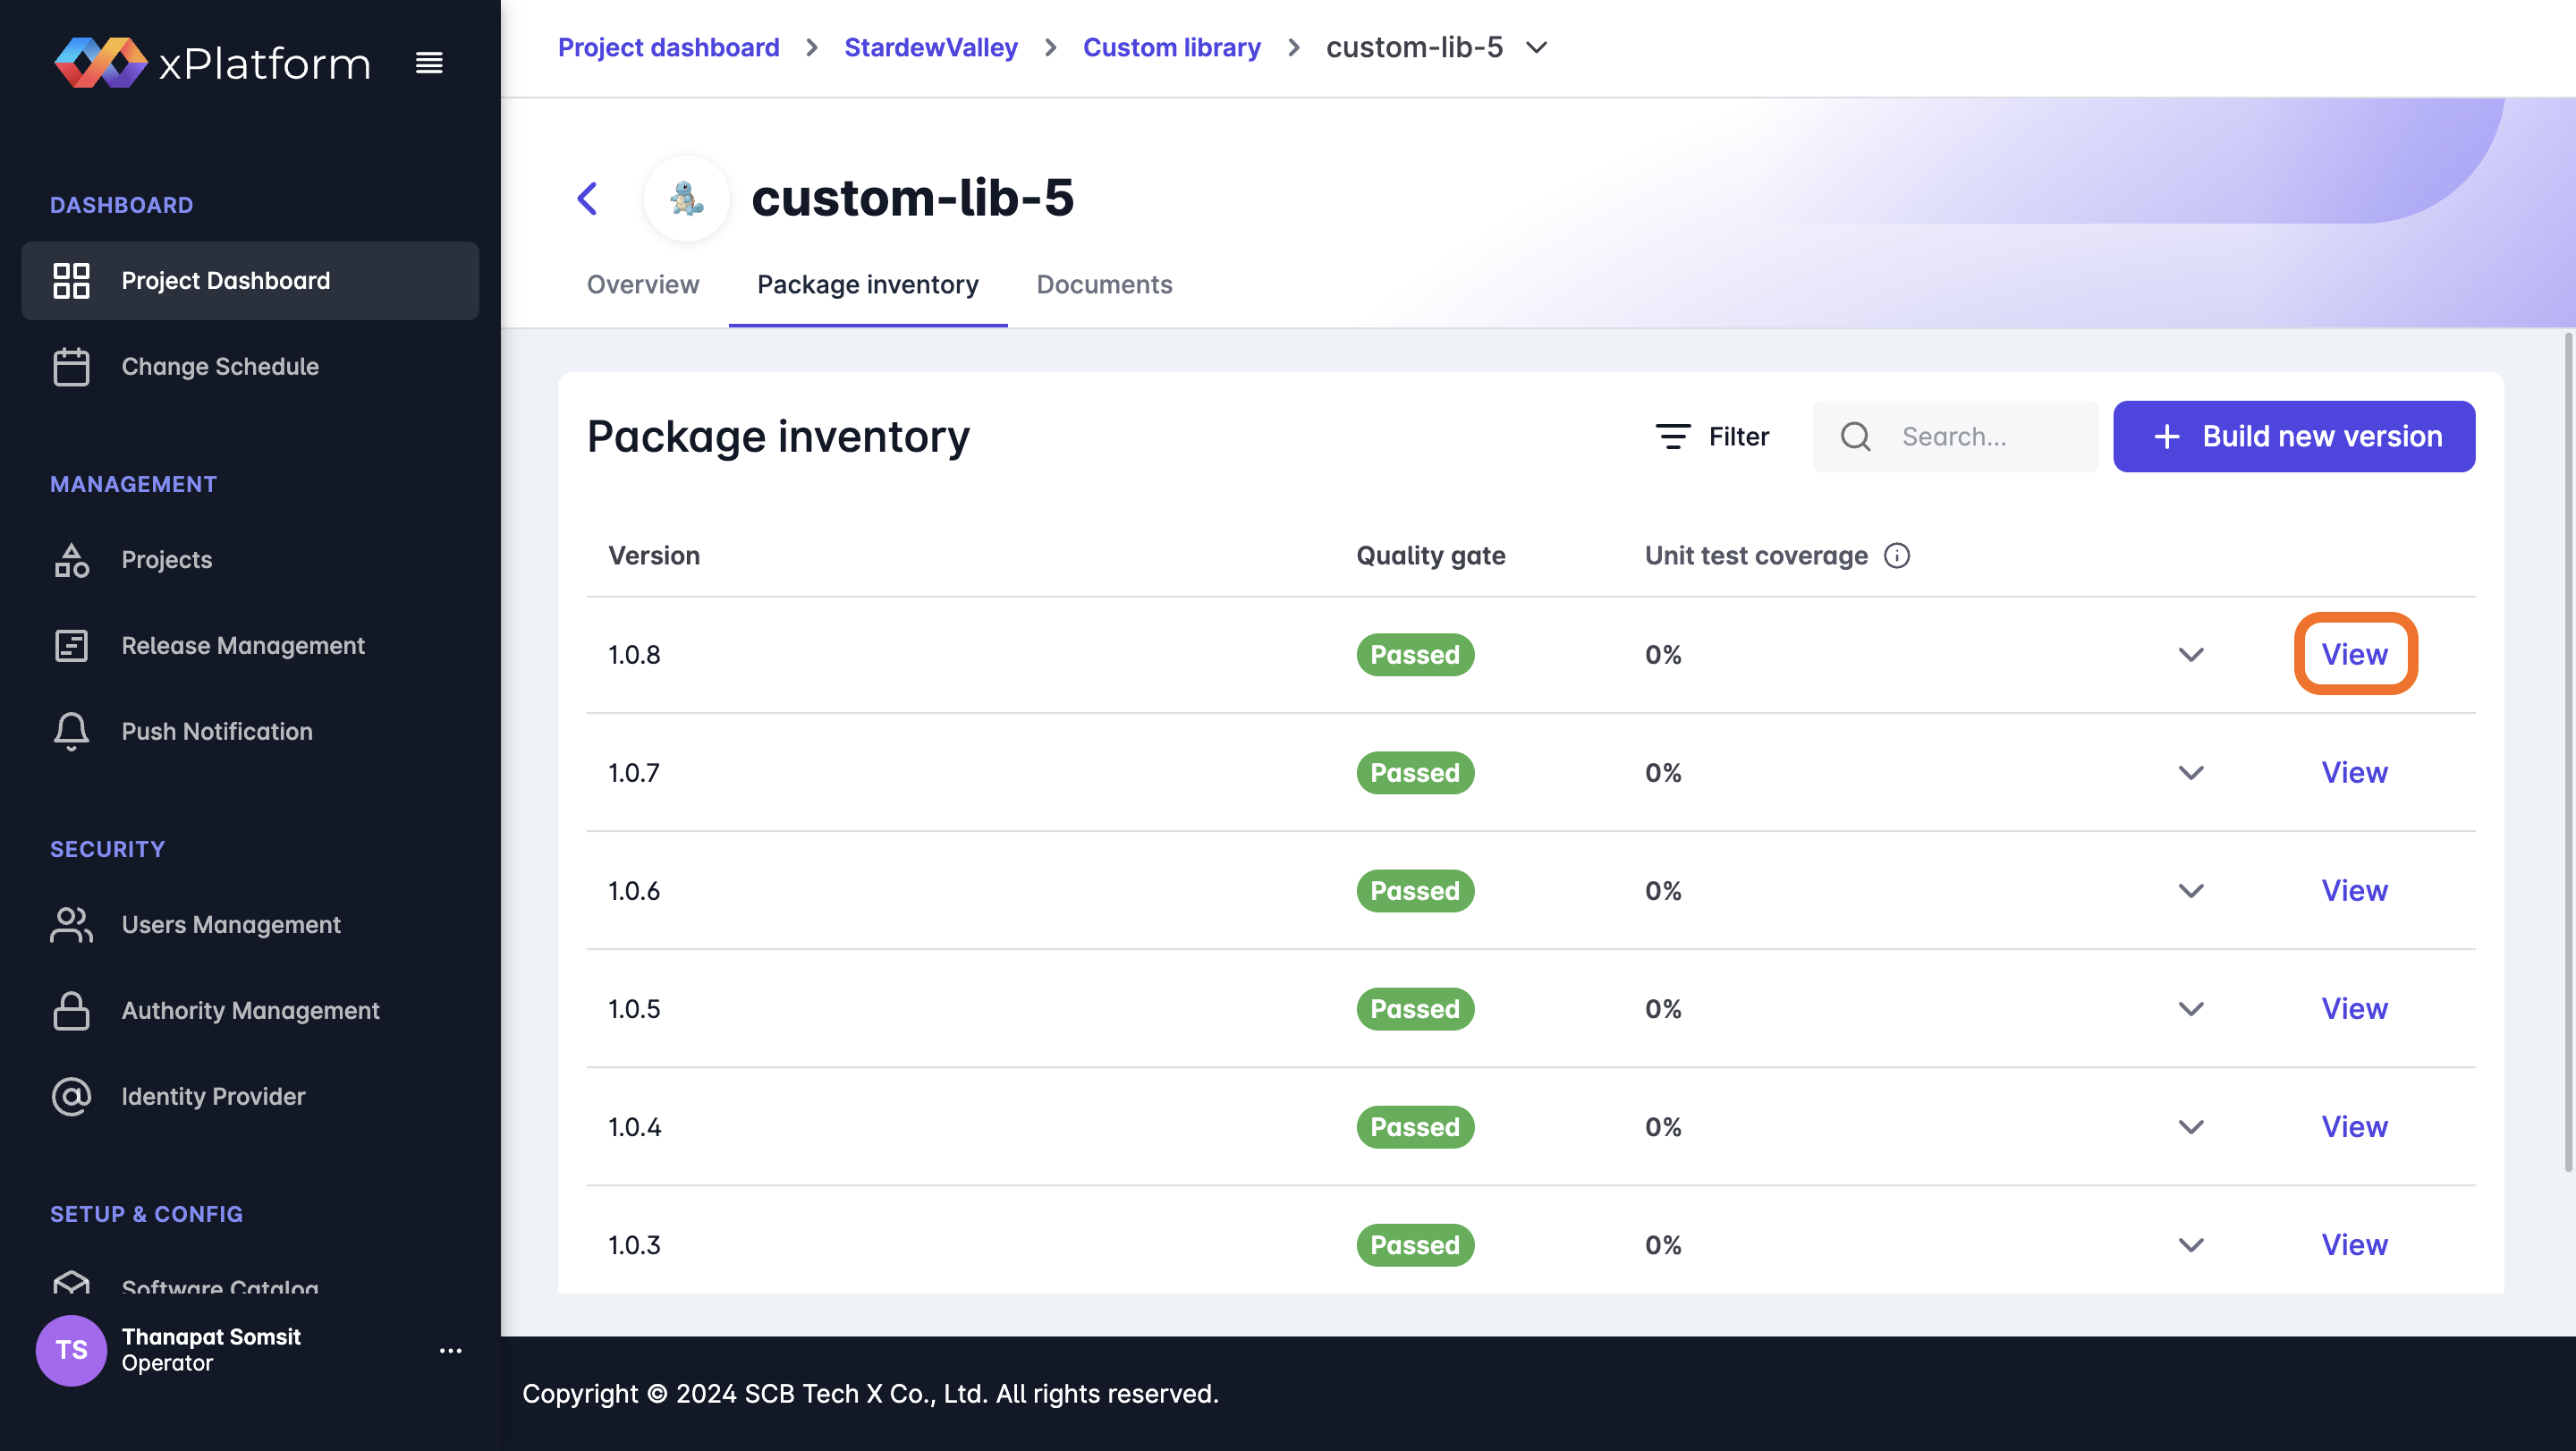
\includegraphics[width=\linewidth]{resources/pages/custom-library/update-library/7.png}
\end{center}

\begin{figure}[H]
    \begin{center}
        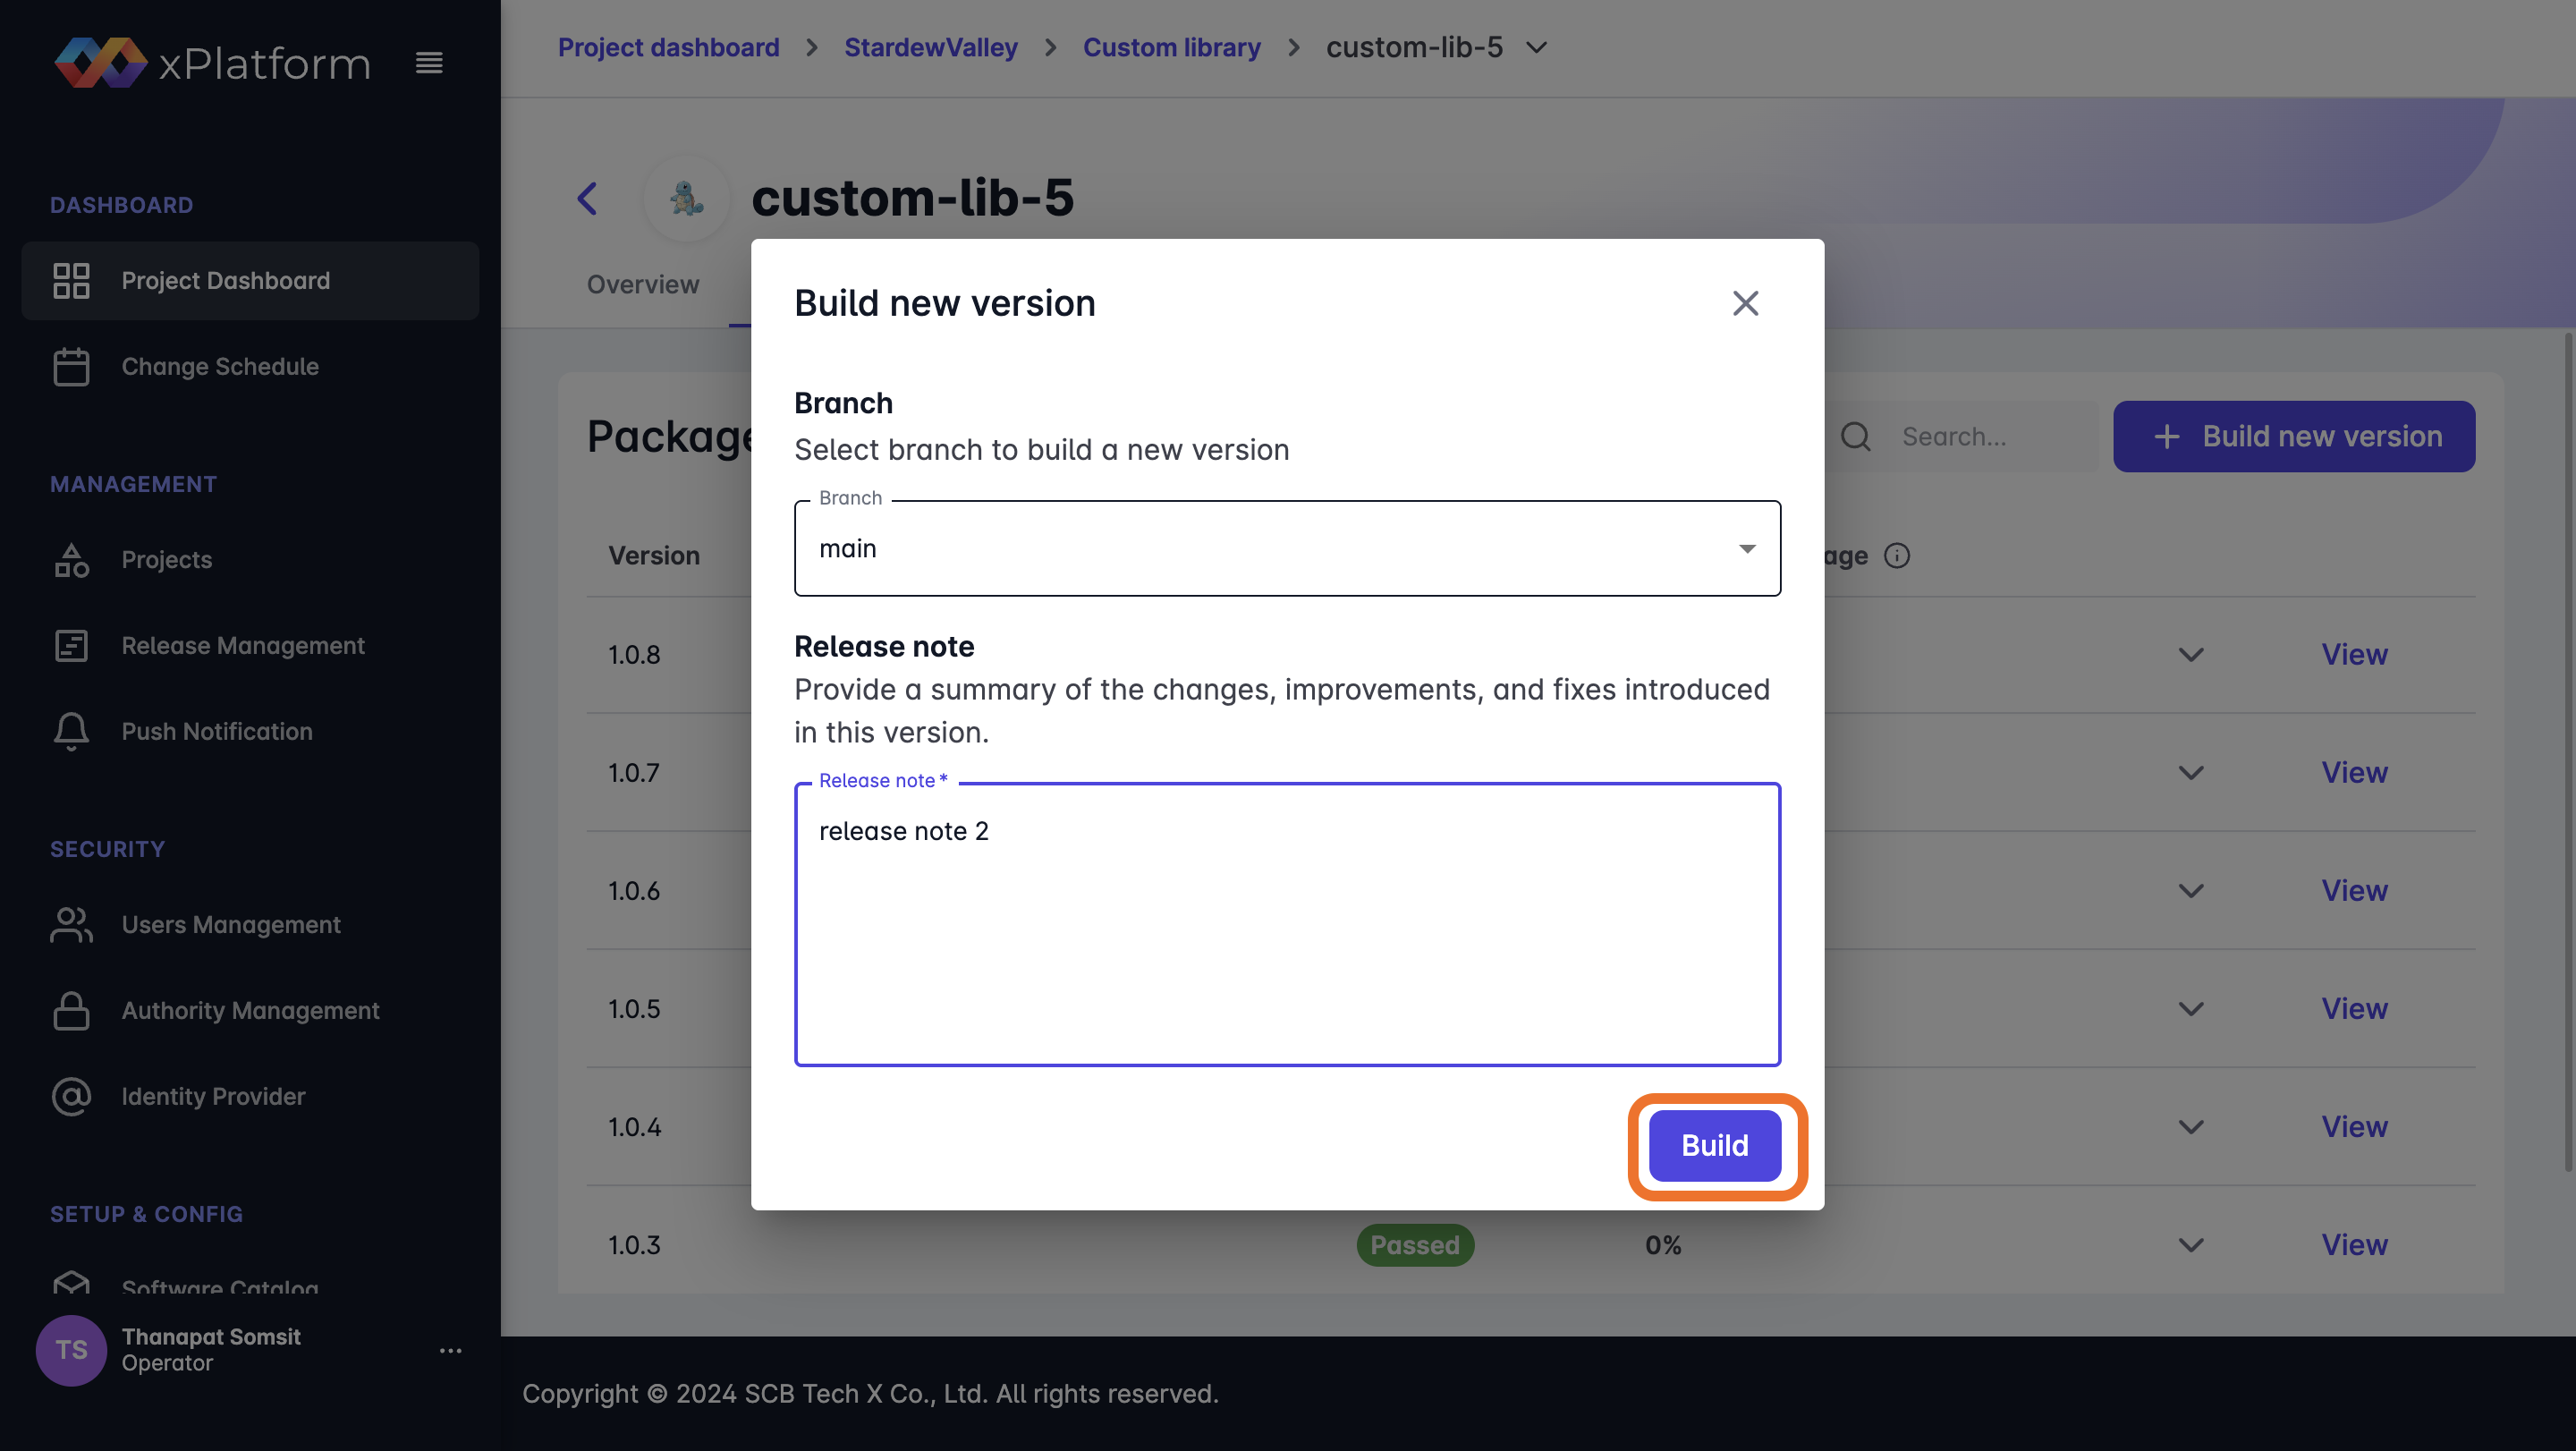
\includegraphics[width=\linewidth]{resources/pages/custom-library/update-library/8.png}
    
        \vspace{1in}
    
        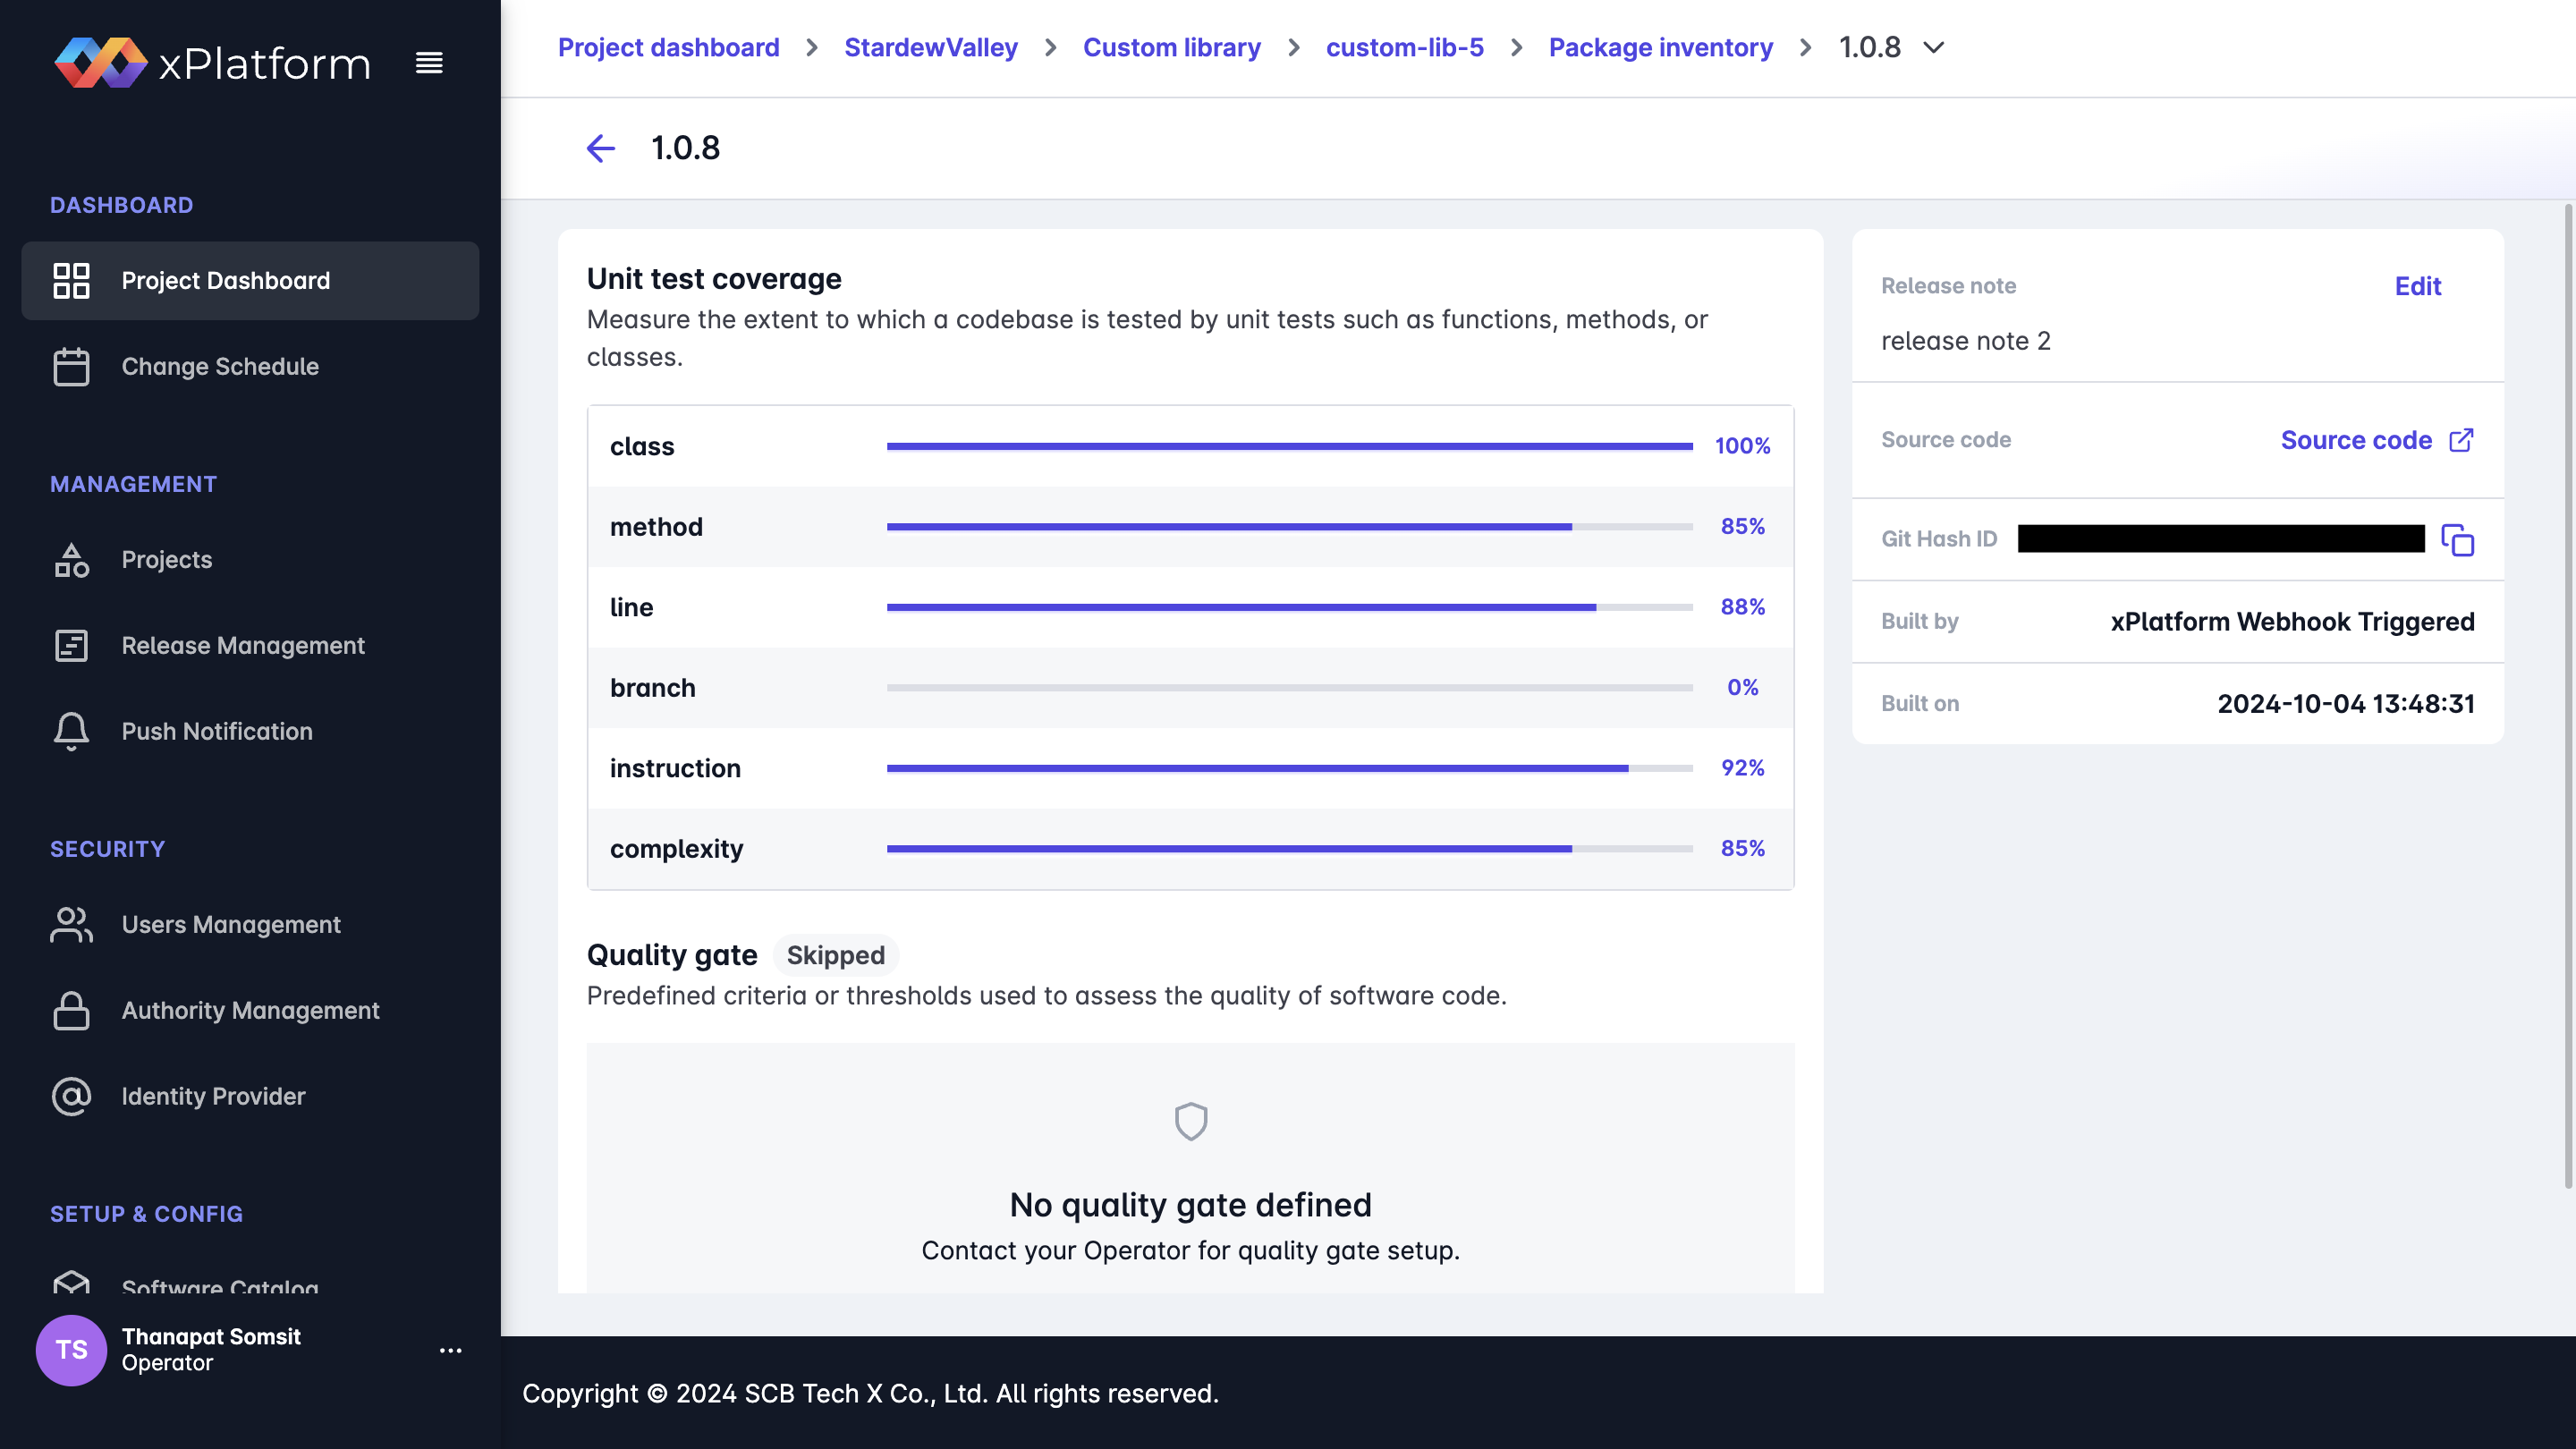
\includegraphics[width=\linewidth]{resources/pages/custom-library/update-library/9.png}
    \end{center}
    \caption[การอัพเดตเวอร์ชัน Custom Library]{การอัพเดตเวอร์ชัน Custom Library}
  \label{fig:update-library}
\end{figure}


\newpage
\section{การใช้งานฟีเจอร์ Documentation}
\begin{center}
    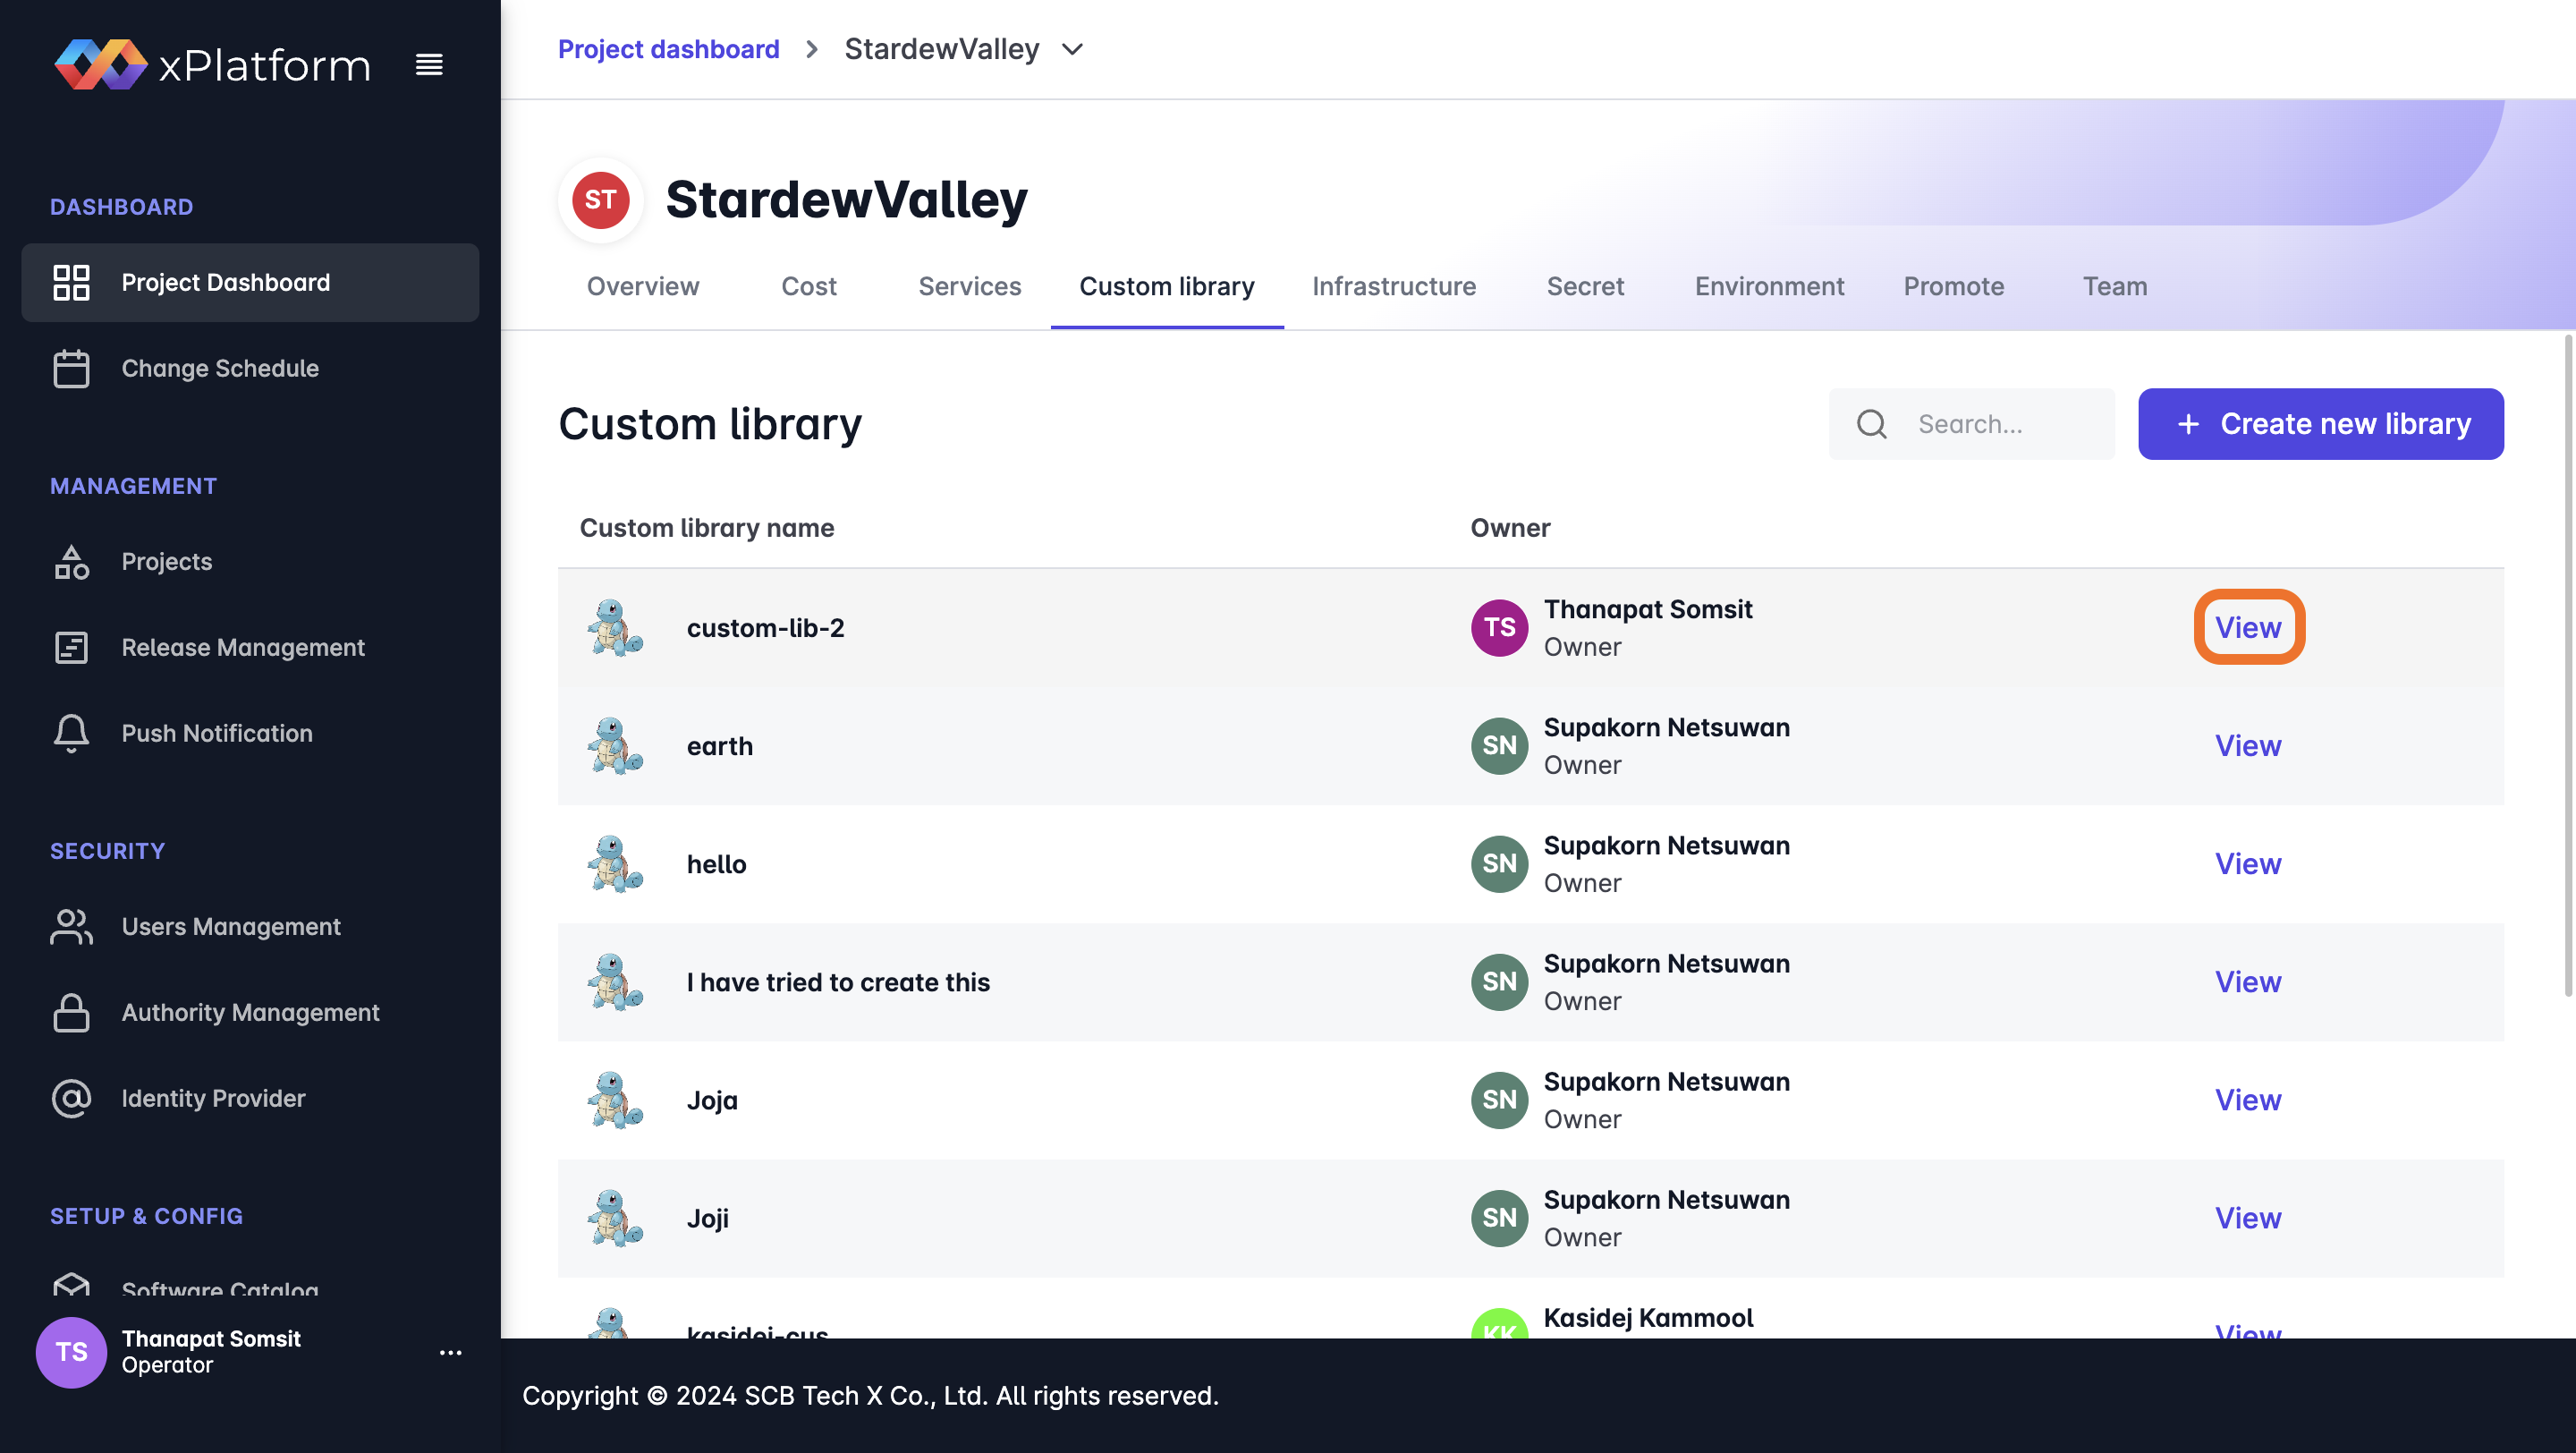
\includegraphics[width=\linewidth]{resources/pages/documentation/1.png}

    \vspace{1in}

    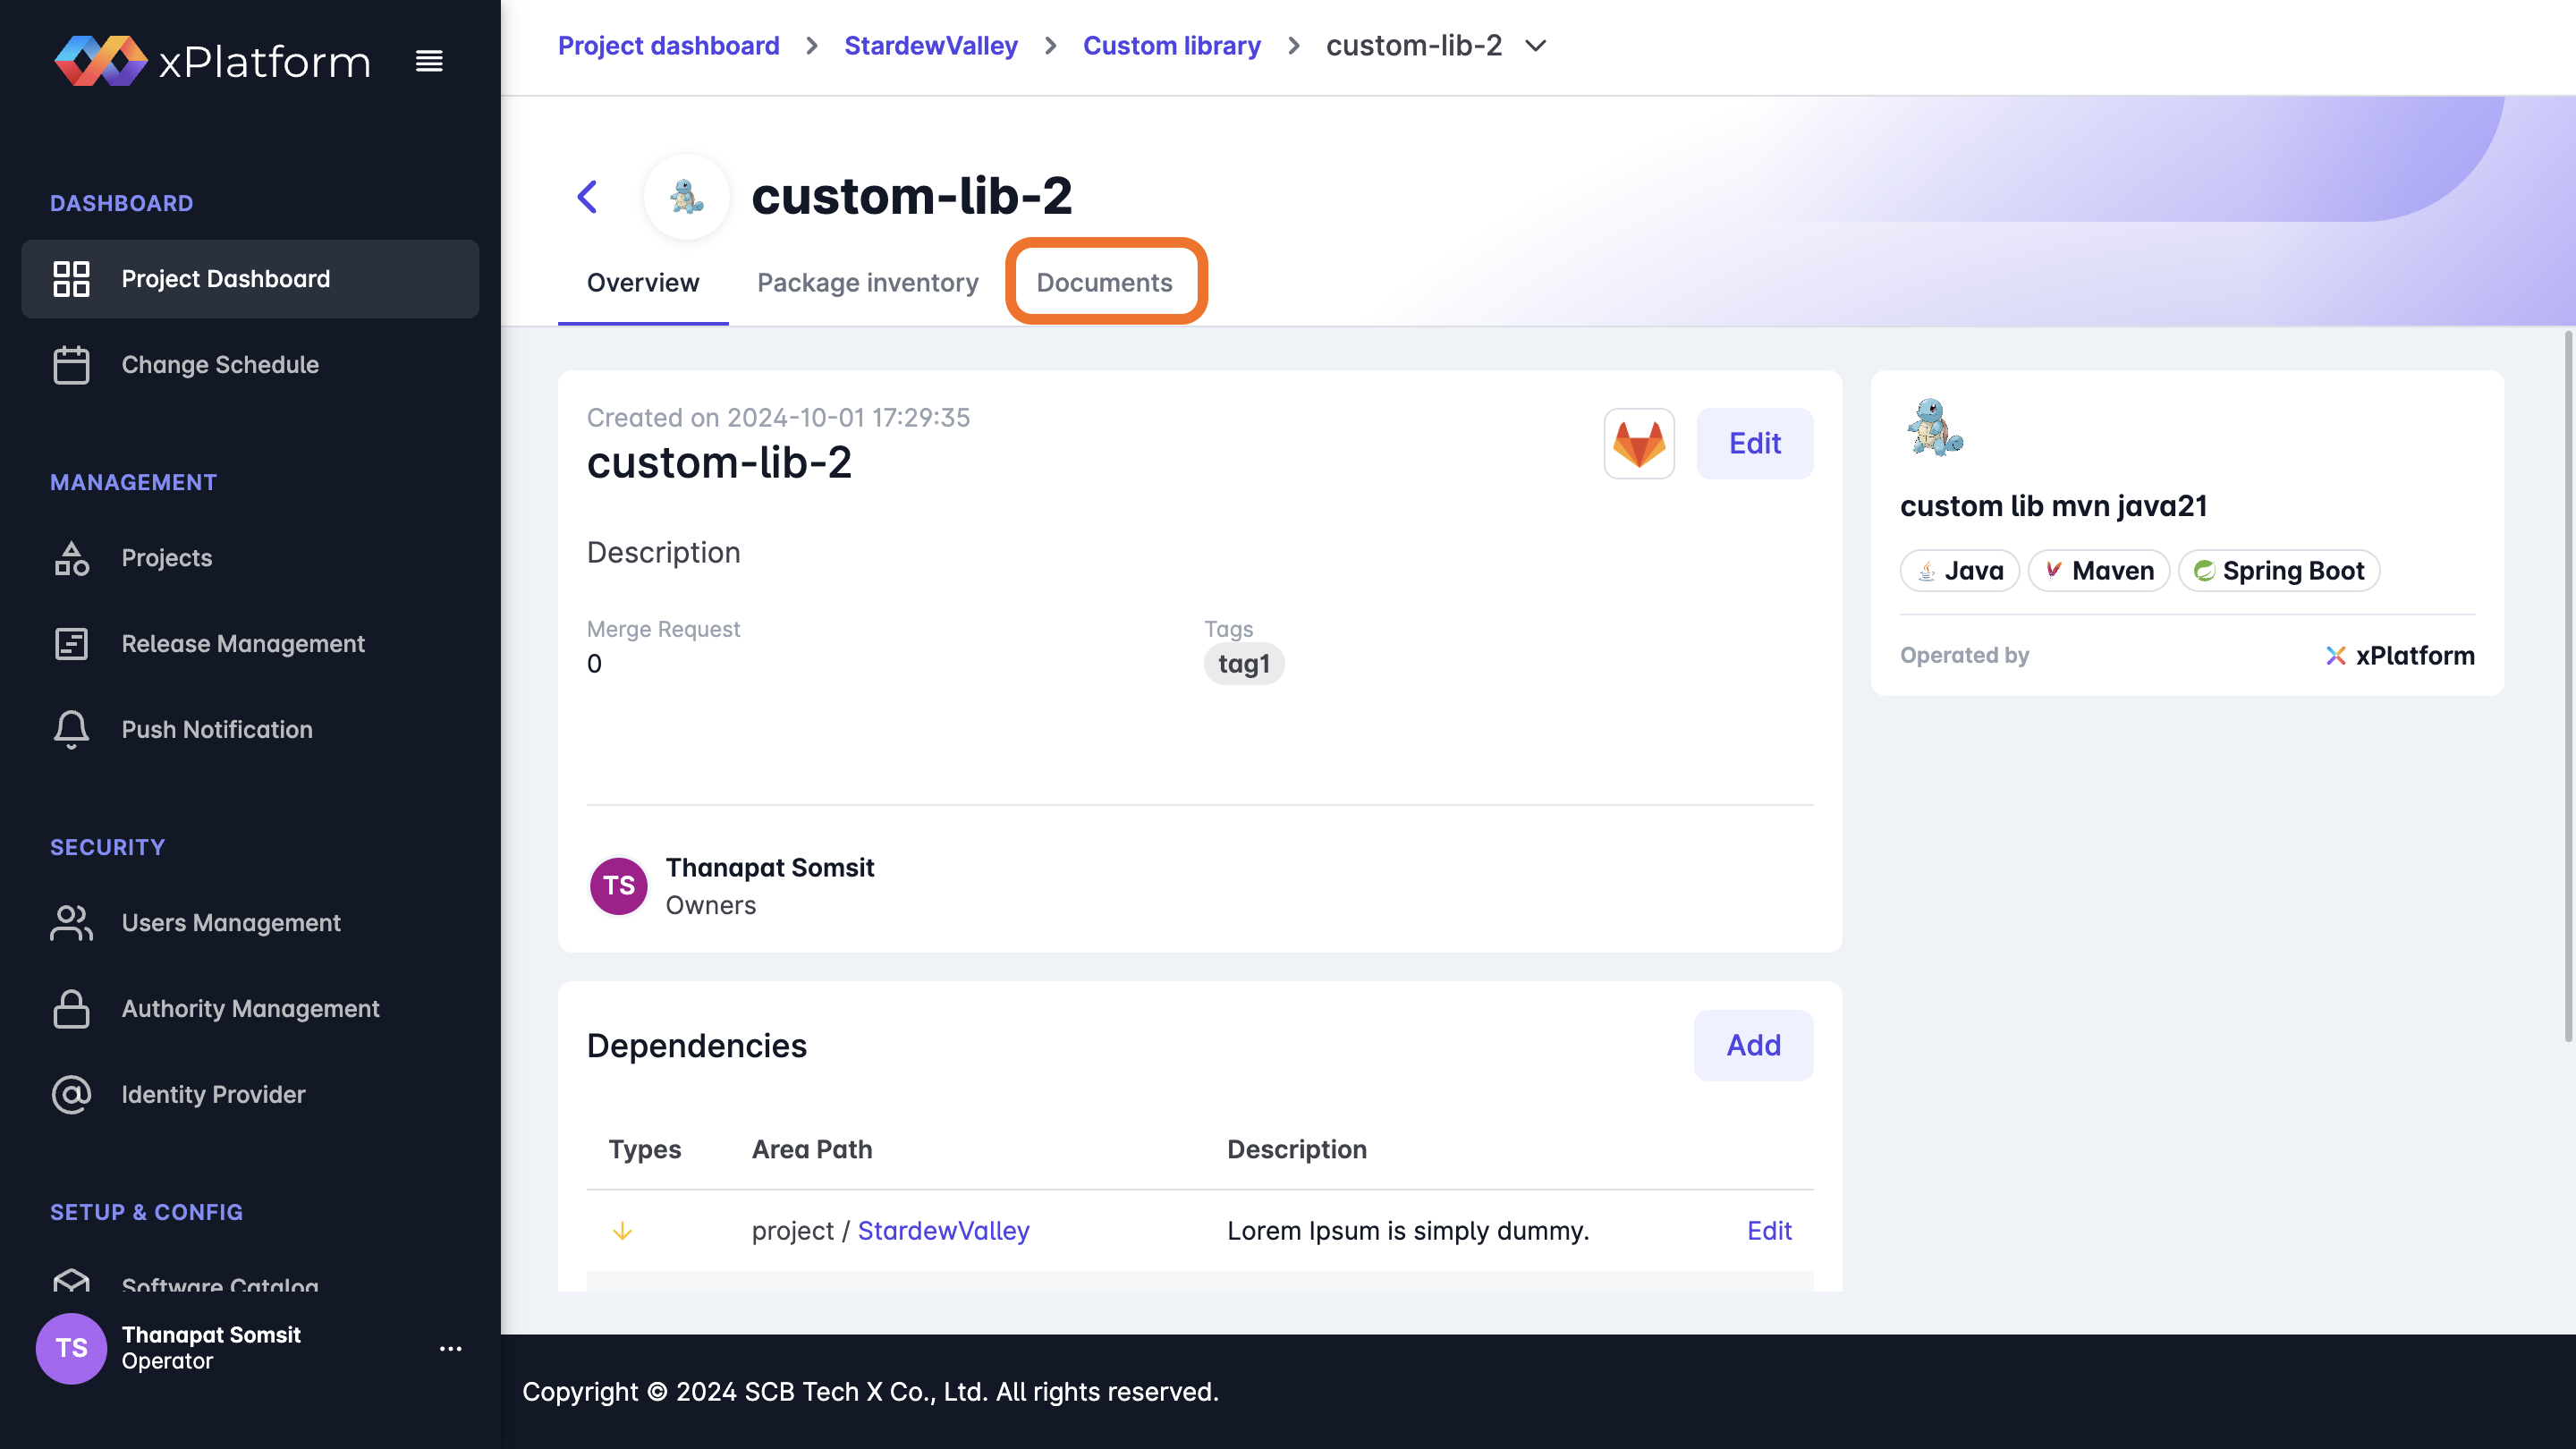
\includegraphics[width=\linewidth]{resources/pages/documentation/2.png}
\end{center}

\begin{figure}[H]
    \begin{center}
        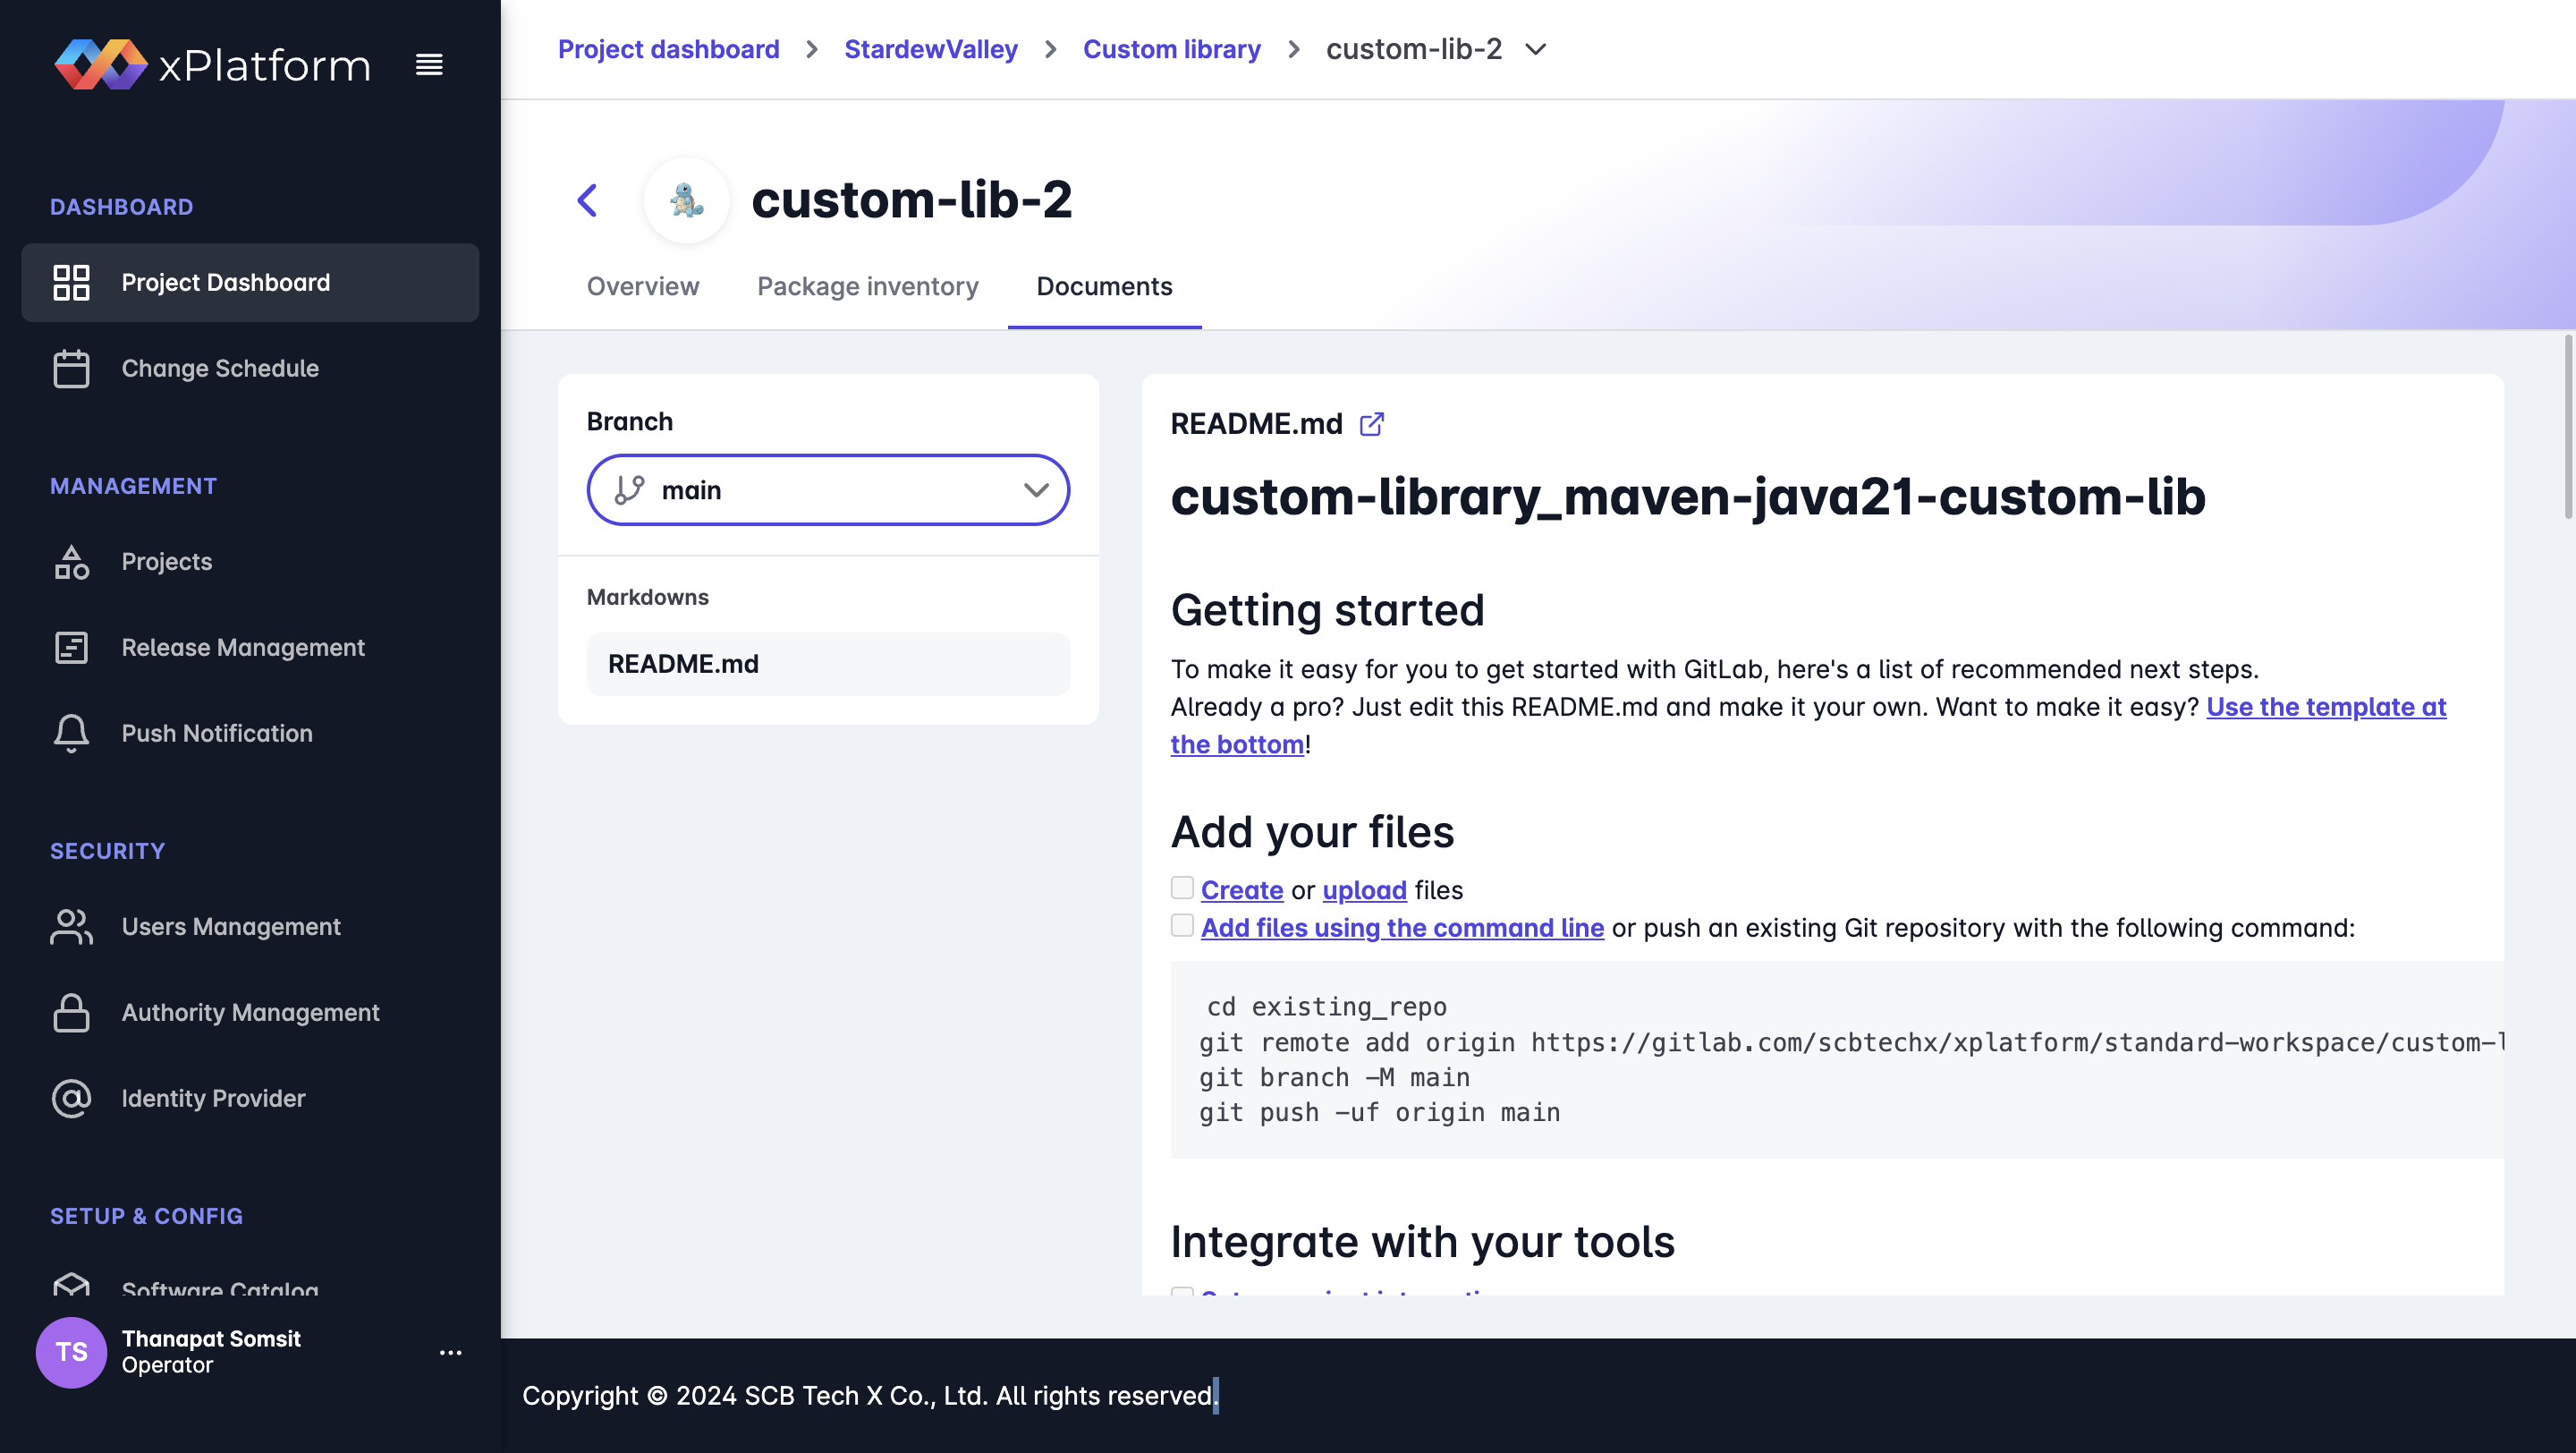
\includegraphics[width=\linewidth]{resources/pages/documentation/3.png}
    \end{center}
    \caption[การใช้งานฟีเจอร์ Documentation]{การใช้งานฟีเจอร์ Documentation}
  \label{fig:documentation}
\end{figure}